\chapterimage{Mavrica.jpg} % Chapter heading image

\chapter{Nelinearna optika}
\label{chap:NLO}
Pri obravnavi svetlobnega valovanja v snovi smo doslej vedno privzeli linearno 
zvezo med polarizacijo in jakostjo električnega polja. To 
je seveda približek, ki je dovolj dober le pri razmeroma majhnih jakostih
polja. Kadar doseže jakost polja velike vrednosti -- in v laserskih snopih
jih nedvomno lahko doseže -- je treba upoštevati tudi višje člene v razvoju. Takrat
govorimo o nelinearni optiki\index{Nelinearna optika}, saj zveza med polarizacijo
in električnim poljem ni linearna. V tem poglavju bomo spoznali zanimive pojave, ki jih 
povzroči nelinearni del polarizacije, med drugim optično 
podvajanje frekvenc, optično usmerjanje, samozbiranje laserskega snopa, 
optične solitone in optično fazno konjugacijo. 

\section{Nelinearna susceptibilnost}
\label{Chap:Chi}
V linearnem približku odziva snovi velja, da je polarizacija snovi\index{Električna polarizacija} 
$\mathbf{P}$ linearna funkcija električne poljske jakosti svetlobe 
$\mathbf{E}$\index{Električno polje!jakost}. Takrat zapišemo (enačba~\ref{eq:PM})
\beq
\mathbf{P} = \mathbf{D} - \varepsilon_0 \mathbf{E} = 
\varepsilon_0 \underline{\epsilon} \cdot\mathbf{E} - \varepsilon_0 \mathbf{E} = 
\varepsilon_0 (\underline{\epsilon} - 1)\cdot\mathbf{E}. 
\eeq
Če uvedemo tenzor linearne susceptibilnosti\index{Susceptibilnost!linearna}
\beq
\chi^{(1)} = \underline{\epsilon} - 1,
\eeq
lahko linearni odziv snovi zapišemo strnjeno kot
\beq
\mathbf{P}_{\mathrm{L}} =  \varepsilon_0 \chi^{(1)} \cdot \mathbf{E}.
\eeq
Ta približek je dober za majhne jakosti električnega polja. Pri večjih poljih
postanejo pomembni tudi členi višjega reda v razvoju polarizacije
po $\mathbf{E}$
\boxeq{8.1}{
\mathbf{P}=\mathbf{P}_{\mathrm{L}}+ \mathbf{P}_{\mathrm{NL}}=
\epsilon_{0} \chi^{(1)}\cdot \mathbf{E}+
\epsilon_{0}\chi^{(2)}:\mathbf{E}\, \mathbf{E}+
\epsilon_{0}\chi^{(3)}\vdots \mathbin \mathbf{E}\mathbin \mathbf{E}\mathbin\mathbf{E} + \dots
}
Vpeljali smo nelinearni susceptibilnosti\index{Susceptibilnost!nelinearna} 
$\chi^{(2)}$ in $\chi^{(3)}$, ki sta tenzorja tretjega in četrtega ranga. 
Za bolj nazorno predstavo izpišimo nelinearna dela še po komponentah
\beq
\left(\mathbf{P}_{\mathrm{NL,2}}\right)_i= \epsilon_{0}\chi^{(2)}_{ijk} \,E_j \,E_k
\label{eq:nlin2}
\eeq
in 
\beq
\left(\mathbf{P}_{\mathrm{NL,3}}\right)_i= \epsilon_{0}\chi^{(3)}_{ijkl} \,E_j \,E_k\, E_l,
\label{eq:nlin3}
\eeq
pri čemer smo uporabili Einsteinov zapis seštevanja po indeksih. Značilne vrednosti
susceptibilnosti v trdnih snoveh so $\chi^{(1)} \sim 1$, 
$\chi^{(2)} \sim 10^{-12}~\textrm{m/V}$ 
in $\chi^{(3)} \sim 10^{-22}$~m$^2$/V$^2$. Obravnavali bomo samo snovi, v katerih
ni izgub in so susceptibilnosti realne.

\begin{definition}
Pokaži, da so gostote svetlobnega toka, pri katerih dosežemo znaten nelinearen 
prispevek k polarizaciji 
 $$\frac{P_{NL}}{P_L} \sim 10^{-6},$$
velikostnega reda 1~MW/cm$^2$. 
Ker so take vrednosti z navadnim svetilom povsem nedosegljive, je bilo mogoče nelinearne
optične pojave opazovati šele po iznajdbi laserjev.
\end{definition}
 
Tenzor $\chi^{(2)}$ je od nič različen le v snoveh, ki nimajo centra inverzije. 
Ker lahko v produktu (enačba~\ref{eq:nlin2}) vrstni red $E_j E_k$ zamenjamo, mora biti
tenzor invarianten na to zamenjavo
\beq
\chi_{ijk} = \chi_{ikj}.
\label{eq:chijk}
\eeq
Vpeljemo poenostavljen zapis, pri katerem prvi indeks prepišemo $(x = 1, y = 2, z = 3)$,
zadnja dva indeksa pa združimo. Dogovorjene oznake so $xx = 1, yy = 2, zz = 3, yz = zy =4, 
xz = zx =5, xy = yx = 6$. Tako na primer $\chi_{xxz}$ zapišemo kot $\chi_{15}$. Namesto
splošnega tenzorja tretjega ranga smo torej uvedli matriko velikosti $3\times6$. 
Vendar koeficienti matrike niso poljubni. Zaradi simetrijskih lastnosti kristala se matrika
poenostavi in navadno je le nekaj komponent različnih od nič. 
Kadar je v snovi absorpcija pri vseh treh frekvencah dovolj majhna, lahko matriko poenostavimo
z dodatnim približkom, tako imenovano  
\index{Kleinmanova domneva} Kleinmanovo domnevo\footnote{D. A. Kleinman, Phys. Rev. 126, 1977 (1962).}.
Ta pravi, da je 
\beq
\chi_{ijk} = \chi_{ikj} = \chi_{kij} = \chi_{kji} = \chi_{jik} = \chi_{jki}.
\eeq
\begin{table}[h!]
 \centering
\begin{tabular}{|c|c|c|c|} \hline  
      Kristal & Grupa & Neničelne komponente tenzorja $\chi$ & Vrednosti ($10^{-12}$~m/V)\\ \hline
      BaTiO\index{BaTiO$_3$}$_3$ & 4mm & $\chi_{xxz} = \chi_{yyz} = \chi_{xzx} = \chi_{yzy} = 
      \chi_{15} = \chi_{24}$  &
	    $\chi_{15} = 42,6$ \\
	      & & $\chi_{zxx} = \chi_{zyy} = \chi_{31} = \chi_{32}$ &  $\chi_{31} = 45,2$ \\
	      & & $\chi_{zzz} = \chi_{33}$ & $\chi_{33} = 16,0$ \\ \hline
      KDP\index{KDP} & 
      $\overline{4}$2m & $\chi_{xyz} = \chi_{yxz} = \chi_{xzy} = \chi_{yzx} = \chi_{14} = \chi_{25}$  &
	    $\chi_{14} = 0,88$ \\
	    & & $\chi_{zxy} = \chi_{zyx} = \chi_{36}$ &  $\chi_{36} =1,12$ \\ \hline
      Telur\index{Telur} & 32 & $\chi_{xxx} = -\chi_{xyy} = -\chi_{yyx} = -\chi_{yxy} =$  & \\
      & &  = $\chi_{11} = -\chi_{12}=-\chi_{26}$  &
	    $\chi_{11} = 1300$ \\
	    & & $\chi_{xyz} = \chi_{xzy} = -\chi_{yxz}= - \chi_{yzx}= \chi_{14} = 
	    -\chi_{25}$ &  $\chi_{14} \approx 0$ 
	    \\ \hline
      LiNbO$_3$\index{LiNbO$_3$} & 3m & $\chi_{xxz} = \chi_{yyz} = \chi_{xzx} = \chi_{yzy} = \chi_{15} = \chi_{24}$  &
	    $\chi_{15} \approx \chi_{31}$ \\
	     & & $\chi_{zxx} = \chi_{zyy} = \chi_{31} = \chi_{32}$ &  $\chi_{31} = -11,9$ \\
	      & & $\chi_{zzz} = \chi_{33}$ & $\chi_{33} = 68,8$ \\
	    & &  $-\chi_{xxy} = - \chi_{xyx} = \chi_{yyy} = -\chi_{yxx}  = $ & \\
	    & & $=-\chi_{16} = \chi_{22}$ = $-\chi_{21}$  &
	    $\chi_{22}  = 5,52$ \\
\hline 
\end{tabular}
  \caption{Koeficienti nelinearne susceptibilnosti za nekaj izbranih snovi}
\label{table:chi}
\end{table}

Poglejmo primer. Vzemimo barijev titanat (BaTiO$_3$)\index{BaTiO$_3$} s točkovno grupo 4mm. To pomeni, da
ima 4-števno os simetrije in dve zrcalni ravnini, od katerih ena preslika $x \to -x$ ali $y \to -y$, 
druga pa $x\to y$ in $y\to x$. Od nič različni elementi susceptibilnosti so tako samo:
\beq
\chi_{xxz} = \chi_{xzx} =   \chi_{yyz} = \chi_{yzy}  ; \quad  \chi_{zzz}; \quad \chi_{zxx} = \chi_{zyy}.   
\eeq
Z upoštevanjem Kleinmanove domneve se število različnih členov še zmanjša in ostaneta le dva
\beq
\chi_{xxz} = \chi_{xzx} = \chi_{yyz} = \chi_{yzy} =\chi_{zxx} = \chi_{zyy} \quad \mathrm{in} \quad \chi_{zzz}.   
\eeq
V tabeli~(\ref{table:chi})\footnote{Izmerjene vrednosti, ki jih najdemo v literaturi, 
se med seboj pogosto znatno razlikujejo.} so navedene izmerjene vrednosti in vidimo, da Kleinmanova
domneva ni povsem točna, ampak zgolj dober približek. 

\section{Nelinearni optični pojavi drugega reda}
\index{Nelinearna optika!drugega reda}
Vzemimo optično nelinearni kristal s $\chi^{(2)} \neq 0$. V smeri pravokotno 
glede na njegovo mejno ploskev naj vpadata dve valovanji s frekvencama
$\omega_{1}$ in $\omega_{2}$. Zaradi nelinearne sklopitve nastajajo v snovi nova 
valovanja z različnimi kombinacijami frekvenc (glej sliko~\ref{fig:nl2}).
\begin{figure}[h]
\centering
\def\svgwidth{140truemm} 
\input{slike/08_nl3.pdf_tex}
\caption{Shematski prikaz nastanka valovanj pri nelinearnih optičnih pojavih drugega reda in spekter
izhodne svetlobe}
\label{fig:nl2}
\end{figure}

Nastanku valovanja pri podvojeni frekvenci pravimo tudi
SHG\index{SHG|see {Optično podvajanje frekvenc}} ({\it Second harmonic 
generation})\index{Optično podvajanje frekvenc}, 
nastanku valovanja pri vsoti frekvenc SFG\index{SFG|see {Generacija vsote frekvenc}}
({\it Sum frequency generation})\index{Generacija vsote frekvenc}, 
nastanku valovanja pri razliki frekvenc DFG\index{DFG|see {Generacija razlike frekvenc}} 
({\it Difference frequency generation})\index{Generacija razlike frekvenc} in pojavu 
statičnega polja pri $\omega = 0$ optično usmerjanje\index{Optično usmerjanje}
({\it Optical rectification}). Oglejmo si nekaj teh pojavov podrobneje. 

Pri močnih vpadnih valovanjih navadna valovna enačba ne zadošča. Pride do pojava
nelinearne polarizacije in valovanje opišemo z nelinearno valovno enačbo\index{Valovna enačba}
\boxeq{8.3}{
\nabla^{2}\mathbf{E}-\frac{\epsilon}{c_0^{2}}{\frac{\partial^2\mathbf{E}}{\partial t^2}}=
\mu_{0}{\frac{\partial^2\mathbf{P}_{\textrm{NL}}}{\partial t^2}}.
}

\begin{definition}
Iz Maxwellovih enačb~(\ref{eq:Maxwell1} do \ref{eq:Maxwell4}) izpelji 
nelinearno valovno enačbo (\ref{8.3}), pri čemer upoštevaj zvezo (\ref{8.1}). 
Pri tem si pomagaj z identiteto
$$
\nabla \times (\nabla \times \mathbf{A}) = \nabla (\nabla \cdot \mathbf{A}) 
- \nabla^2 \mathbf{A}.
$$
\end{definition} 

Nehomogene valovne enačbe v splošnem ne znamo rešiti in se moramo zateči k približkom.
Prva poenostavitev, ki jo bomo naredili, je omejitev na vzporedna vpadna žarka,
ki se širita v smeri osi $z$. Poleg tega se bomo omejili na izračun samo enega
nastalega valovanja in privzeli, da je neodvisno od drugih nastalih valovanj.
Ta omejitev ni huda. Dokler sta namreč amplitudi valovanj pri vsoti in razliki
frekvenc majhni, ju lahko obravnavamo vsako posebej. Ni sicer nujno,
da sta obe nastali amplitudi vedno majhni, vendar je lahko, kot bomo videli kasneje, 
le eno valovanje naenkrat po jakosti primerljivo z vpadnim. 

V snovi so tako prisotna tri valovanja:
dve vpadni in tretje, novo nastalo
\begin{eqnarray}
\mathbf{E}_{1} & = & \frac{\mathbf{e}_{1}}{2}\left[A_{1}(z)\, 
e^{i(k_{1}z-\omega_{1}t)}+A_{1}^{*}(z)\, e^{-i(k_{1}z-\omega_{1}t)}\right]\nonumber \\
\mathbf{E}_{2} & = & \frac{\mathbf{e}_{2}}{2}\left[A_{2}(z)\, 
e^{i(k_{2}z-\omega_{2}t)}+A_{2}^{*}(z)\, e^{-i(k_{2}z-\omega_{2}t)}\right]\nonumber \\
\mathbf{E}_{3} & = & \frac{\mathbf{e}_{3}}{2}\left[A_{3}(z)\, 
e^{i(k_{3}z-\omega_{3}t)}+A_{3}^{*}(z)\, e^{-i(k_{3}z-\omega_{3}t)}\right].
\end{eqnarray}
Polja smo zapisali v realni obliki, to je s kompleksno konjugiranimi
deli, saj valovna enačba (\ref{8.3}) ni linearna. Upoštevali smo tudi,
da so zaradi nelinearnih pojavov amplitude funkcije kraja, za
katere pa lahko privzamemo, da se le počasi spreminjajo. Njihova kompleksna vrednost
dopušča pojav dodatnega faznega zamika. Za valovna
števila velja $k_{n}^{2}=\epsilon_{n}\omega_n^{2}/c_0^{2}$,
pri čemer je $\epsilon_{n}$ dielektrična konstanta pri frekvenci
$\omega_{n}$ in polarizaciji $\mathbf{e}_{n}$, indeks $n = 1...3$ pa označuje
valovanje. S tem vsako od treh valovanj
pri konstantni amplitudi reši linearni del valovne enačbe. 

Naša naloga
je ugotoviti, kako se zaradi nelinearnosti spreminjajo amplitude posameznih valovanj.
Nastavek za polje, ki bo rešil nelinearno valovno enačbo, je tako
\beq
\mathbf{E}(z,t) = \sum_{n=1}^3 \frac{\mathbf{e}_{n}}{2}\left[A_{n}(z)\, 
e^{i(k_{n}z-\omega_{n}t)}+A_{n}^{*}(z)\, e^{-i(k_{n}z-\omega_{n}t)}\right].
\label{eq:nlnastavek}
\eeq
Izračunajmo najprej 
\begin{equation}
\nabla^{2}\mathbf{E}=-\sum_{n=1}^3 \frac{\mathbf{e}_{n}}{2}\left[k_{n}^{2}A_{n}(z)-2ik_{n}
\frac{dA_{n}(z)}{dz}\right]\, e^{i(k_{n}z-\omega_{n}t)}+\mbox{ k. k.}
\label{8.5}
\end{equation}
S k. k. smo označili kompleksno konjugirani del. Upoštevali smo,
da se amplituda $A_{n}(z)$ le počasi spreminja s krajem in smo zato njen
drugi odvod zanemarili.
Izračunamo še drugi odvod po času 
\begin{equation}
\frac{\partial^2\mathbf{E}}{\partial t^2}=\sum_{n=1}^3 \frac{\mathbf{e}_{n}}{2}
\left(-\omega_n^2\right) \left[A_{n}(z)\, e^{i(k_{n}z-\omega_{n}t)}+\mbox{ k. k.}\right].
\label{8.5a}
\end{equation}
Nelinearna polarizacija vsebuje produkte polj, ki nihajo z vsemi možnimi
vsotami in razlikami parov frekvenc $\omega_{1}$, $\omega_{2}$ in
$\omega_{3}$
\begin{multline}
\mathbf{P}_{\mathrm{NL}}= \epsilon_{0}\chi^{(2)}:\mathbf{E}\, \mathbf{E} =
\varepsilon_0 \sum_{n=1}^3 \sum_{m=1}^3 
 \left( \frac{1}{4} \chi^{(2)}:\mathbf{e}_{n}\,\mathbf{e}_{m}\right) 
 A_{n}(z)\,A_{m}(z) e^{i(k_{n}+k_{m})z-i(\omega_{n}+\omega_{m})t}+  \\
\left( \frac{1}{4} \chi^{(2)}:\mathbf{e}_{n}\,\mathbf{e}_{m}\right)
A_{n}(z)\,A_{m}^*(z) e^{i(k_{n}-k_{m})z-i(\omega_{n}-\omega_{m})t}+ \mathrm{k. k.}
\label{8.5b}
\end{multline}
Če želimo, da je valovna enačba~(\ref{8.3}) izpolnjena ob vsakem času $t$, se morajo
ujemati izrazi pri istih časovnih odvisnostih, to je pri istih frekvencah. Izberimo
najprej člene pri $\omega_n = \omega_3$ in $\omega_3 = \omega_1 + \omega_2$. Dobimo
\beq
ik_{3}\mathbf{e}_{3}\frac{dA_{3}}{dz}e^{ik_{3}z}=-\frac{\mu_{0} 
\varepsilon_0 \omega_{3}^{2}}{4}\chi:\mathbf{e}_{1}\mathbf{e}_{2}\,A_{1}\,A_{2}e^{i(k_{1}+k_{2})z}.
\label{8.7}
\eeq
Množimo še obe strani skalarno z $\mathbf{e}_{3}$, upoštevajmo zvezo med $k_{3}$ in $\omega_{3}$
in ravnajmo podobno še za drugi dve valovanji. Tako dobimo sistem sklopljenih
enačb za amplitude valovanj v optično nelinearnem sredstvu
\boxeq{eq:nlAz}{
\frac{dA_{3}}{dz} &= \frac{i\omega_{3}\chi_{ef}}{4c_0 n_3} A_{1}\, A_{2}\, e^{-i\Delta kz}\\
\frac{dA_{2}}{dz} &= \frac{i\omega_{2}\chi_{ef}}{4c_0 n_2} A_{1}^*\, A_{3}\, e^{i\Delta kz}\\
\frac{dA_{1}}{dz} &= \frac{i\omega_{1}\chi_{ef}}{4c_0 n_1} A_{2}^*\, A_{3}\, e^{i\Delta kz}\label{eq:nlA3}.
}
Pri tem je 
\beq
\chi_{ef}=\mathbf{e}_{3}\cdot\chi:\,\mathbf{e}_{1}\,\mathbf{e}_{2} = 
\sum_{ijk} \chi_{ijk} e_{3i} e_{1j} e_{2k}.
\label{eq:chicomp}
\eeq
Ker ni nujno, da so polarizacijski vektorji vzporedni s koordinatnimi osmi, tudi $\chi_{ef}$ 
niso čiste kartezične komponente tenzorja nelinearne susceptibilnosti. 

Z $\Delta k$ smo označili razliko valovnih vektorjev
\beq
\Delta k = k_{3}-k_{1}-k_{2}.
\eeq
Čeprav je $\omega_{3}-\omega_{2}-\omega_{1}=0$, je $\Delta k$ navadno različen od nič zaradi 
frekvenčne disperzije lomnega količnika. Videli bomo, da je to ključnega pomena 
za vrsto nelinearnih optičnih pojavov. Dobljeni sistem sklopljenih diferencialnih enačb opisuje več pojavov, 
odvisno od začetnih pogojev in relativnih intenzitet valovanj. Mi si bomo ogledali le nekaj
najpomembnejših primerov.
\begin{definition}
Pokaži, da nastavek za polje v nelinearni snovi (enačba~\ref{eq:nlnastavek}) reši nelinearno
valovno enačbo (\ref{8.3}), in pokaži, da spreminjanje amplitude posameznih valovanj 
ustreza enačbam~(\ref{eq:nlAz}-\ref{eq:nlA3}).
\end{definition}

\section{Optično podvajanje frekvenc}

Obravnavajmo optično nelinearno sredstvo, na katerega vpadata valovanji $E_1$ in $E_2$.
Naj bosta frekvenci vpadnih valovanj enaki $\omega_{1}=\omega_{2}=\omega$, valovanji
pa razlikujemo zaradi možnosti dveh različnih polarizacij. Takrat je $\omega_{3}=2\omega$
in govorimo o najpreprostejšem in tudi najpomembnejšem optičnem nelinearnem 
pojavu~\textendash~podvajanju 
frekvence\index{Optično podvajanje frekvenc}. 
Pogosto ga uporabljamo za pridobivanje laserskih snopov pri krajših valovnih dolžinah, na primer
pri Nd:YAG laserju\index{Laser!Nd:YAG}, ko infrardeče izhodno valovanje (1064~nm) 
pretvorimo v vidno svetlobo zelene barve (532~nm). 

Zanima nas, kako se $A_{3}(z) = A_{2\omega}(z)$ spreminja vzdolž nelinearnega kristala
pri začetnem pogoju $A_{2\omega}(0)=0$.
Privzemimo še, da se pretvori le manjši del vpadnega energijskega toka,
tako da sta amplitudi $A_{1}=A_{2}=A_0$ približno konstantni. Tedaj lahko
enačbo za $A_{3}(z)$ (enačba~\ref{eq:nlAz}) brez težav integriramo do dolžine kristala $L$ in dobimo
\begin{equation}
A_{2\omega}(L)=\frac{i\omega \chi_{ef} A_0^2}{2c_0 n_{2\omega}}
\,e^{-i\Delta kL/2}\, \frac{\sin\left(\frac{\Delta k L}{2}\right)}{\frac{\Delta kL}{2}}L,
\label{8.9}
\end{equation}
kjer smo z $n_{2\omega}$ označili lomni količnik pri dvojni frekvenci.
Iz tega izraza izračunamo izhodno gostoto svetlobnega toka pri dvojni
frekvenci 
\begin{equation}
j_{2\omega}(L) =\frac{1}{2}\epsilon_{0}n_{2\omega}c_0|A_3|^2 = 
\frac{\omega^2 \chi_{ef}^2}{2 n_{2\omega} n_\omega^2c_0^3\varepsilon_0} j_\omega^2 L^2
\left(\frac{\sin\left(\frac{\Delta k L}{2}\right)}{\frac{\Delta kL}{2}}\right)^2.
\label{8.10}
\end{equation}
Gostota energijskega toka frekvenčno podvojene svetlobe torej narašča s kvadratom
intenzitete vpadne svetlobe. Naj bo $S$ presek snopa. Potem je razmerje med 
energijskim tokom pri podvojeni in osnovni frekvenci oziroma izkoristek pretvorbe
\boxeq{8.11}{
\frac{P_{2\omega}}{P_{\omega}}=
\frac{\omega^2 \chi_{ef}^2}{2 S n_{2\omega} n_\omega^2c_0^3\varepsilon_0} P_\omega L^2
\left(\frac{\sin\left(\frac{\Delta k L}{2}\right)}{\frac{\Delta kL}{2}}\right)^2.
}

\begin{remark}
Pri izpeljavi frekvenčnega podvajanja iz enačb za nelinearne pojave drugega
reda (enačbe~\ref{eq:nlAz}-\ref{eq:nlA3}) moramo biti pazljivi. 
Tukaj smo uporabili splošne enačbe in tako privzeli, da je 
vpadno valovanje sestavljeno iz dveh ločenih valovanj s frekvenco $\omega$
z intenziteto $j_\omega$. Lahko pa frekvenčno podvajanje obravnavamo
z enim vpadnim valovanjem s frekvenco $\omega$ in intenziteto $2j_\omega$, 
ki nelinearno interagira samo s sabo. Takrat je zapis enačb za predfaktor
drugačen, končen rezultat pa seveda enak. 
\end{remark}

V izrazih (\ref{8.10}) in (\ref{8.11}) nastopa 
faktor $\sin^{2}(\Delta kL/2)/(\Delta kL/2)^{2}$ (slika~\ref{fig:shg2}). 
Zaradi njega je na poti, ki je daljša od $\pi /\Delta k$, stopnja pretvorbe zelo majhna.
\begin{figure}[h]
\centering
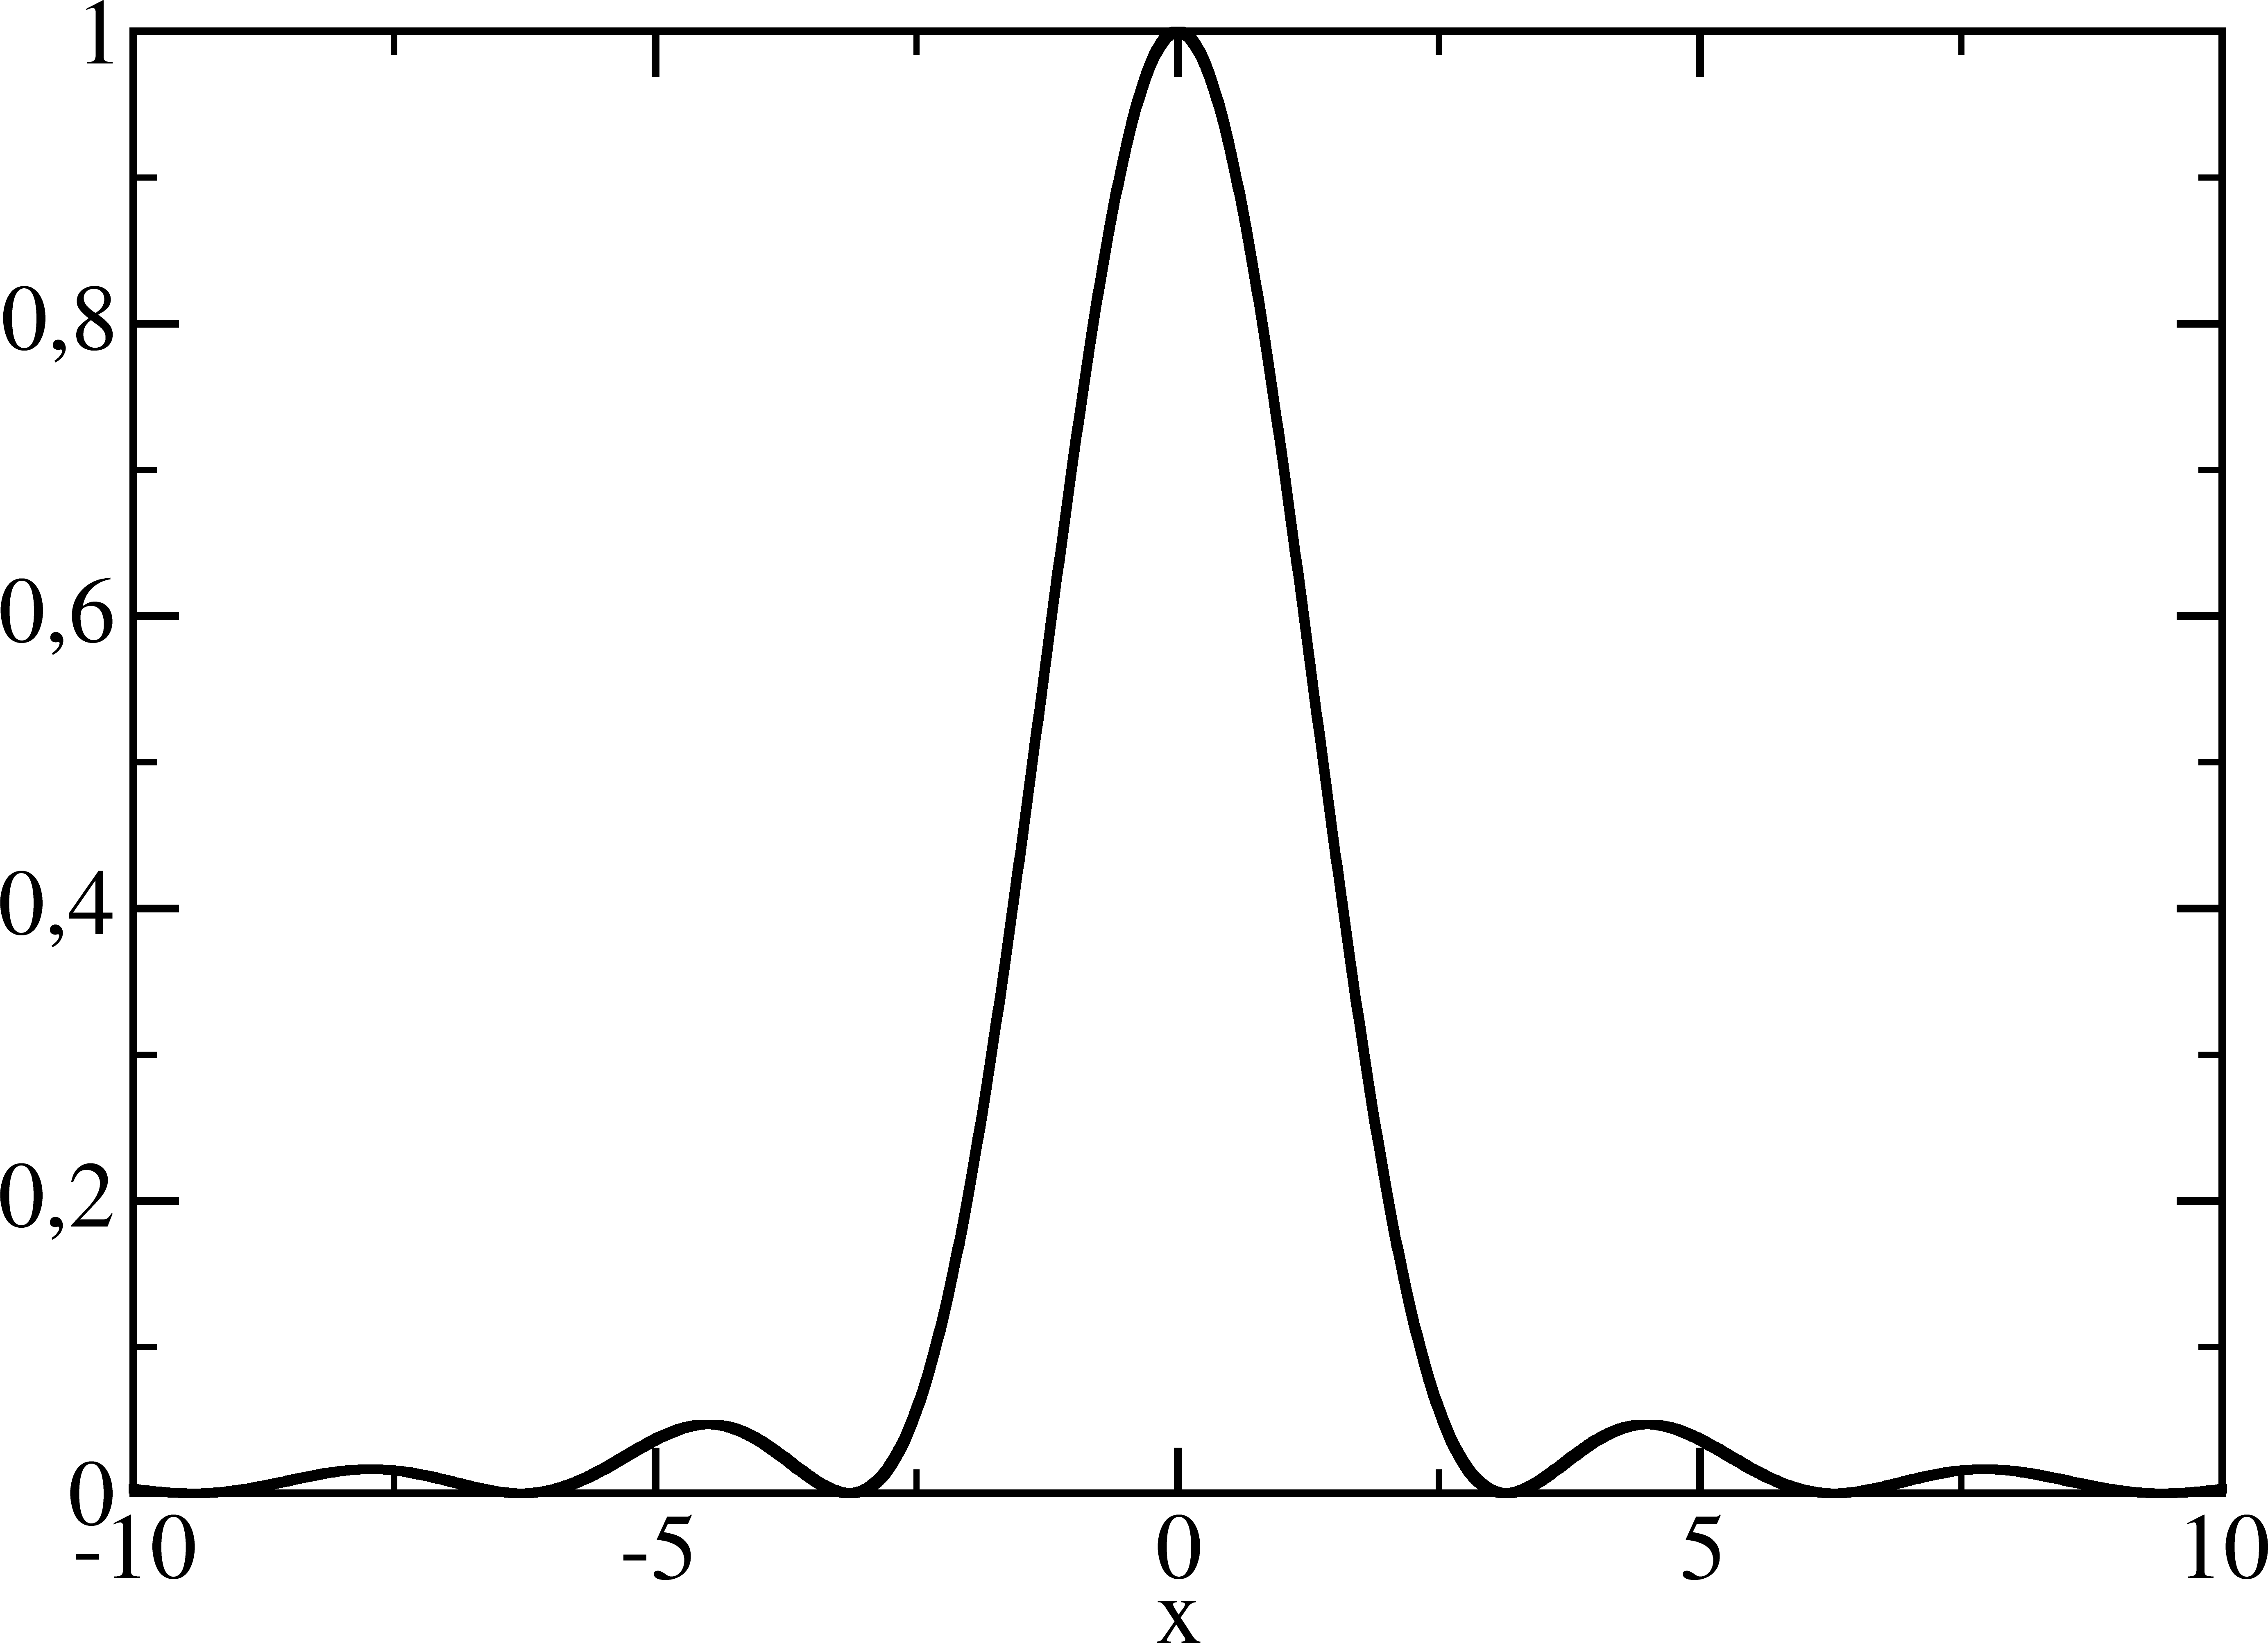
\includegraphics[width=7truecm]{slike/08_shg2.png}
\caption{Izkoristek pretvorbe v frekvenčno podvojeno valovanje je 
sorazmeren s funkcijo $(\sin(x)/x)^2$,
pri čemer je $x = \Delta k L/2$.}
\label{fig:shg2}
\end{figure}

Poglejmo primer. Faktor $\Delta k$ je različen od nič zaradi odvisnosti
lomnih količnikov od frekvence. V KH$_{2}$PO$_{4}$\index{KDP} je 
redni lomni količnik pri 1000 nm 1,496, pri 500 nm pa 1,514. Vrednost, pri kateri
pade intenziteta frekvenčno podvojenega valovanja na nič
$L_{c}=\pi /\Delta k$, je tako le okoli 30 mikrometrov. Na večjih dolžinah
postane stopnja pretvorbe zanemarljivo majhna.

Za visok izkoristek pretvorbe v frekvenčno podvojeno valovanje je torej 
pomembno, da se faze čim bolj ujemajo in da je $\Delta k = 0$. 
Takrat je vrednost faktorja $\sin(\Delta kL/2)/(\Delta kL/2)$ največja in izkoristek 
pretvorbe narašča sorazmerno s kvadratom dolžine
\beq
\frac{P_{2\omega}}{P_{\omega}}=
\frac{\omega^2 \chi_{ef}^2}{2 S n_{2\omega} n_\omega^2c_0^3\varepsilon_0} P_\omega L^2.
\eeq
Za uporabno pretvorbo v frekvenčno podvojeno valovanje je torej treba doseči 
fazno ujemanje valovnih vektorjev\index{Ujemanje faz} 
pri osnovni in podvojeni frekvenci. Kako to naredimo,
bomo spoznali v prihodnjem razdelku.

\begin{definition}
\label{deplet}
Vemo, da intenziteta frekvenčno podvojenega valovanja narašča sorazmerno s
kvadratom dolžine kristala. Takšna odvisnost velja le, če je intenziteta valovanja
pri podvojeni frekvenci bistveno manjša od intenzitete vpadnega valovanja, 
oziroma $A_3 \ll A_1, A_2$. Pokaži, da v nasprotnem primeru intenziteta frekvenčno
podvojenega valovanja $j_{2\omega}(L)$ narašča kot
\beq
j_{2\omega} (L) = j_0 \tanh^2 \left(\chi_{ef}\omega \sqrt{\frac{j_0}
{2 n_3 n_1^2 c_0^3 \varepsilon_0}} L\right),
\eeq
pri čemer je $j_0$ vpadna intenziteta valovanja pri osnovni frekvenci. Namig: upoštevaj, 
da se celotna energija ohranja.
\end{definition}

\begin{figure}[h]
\centering
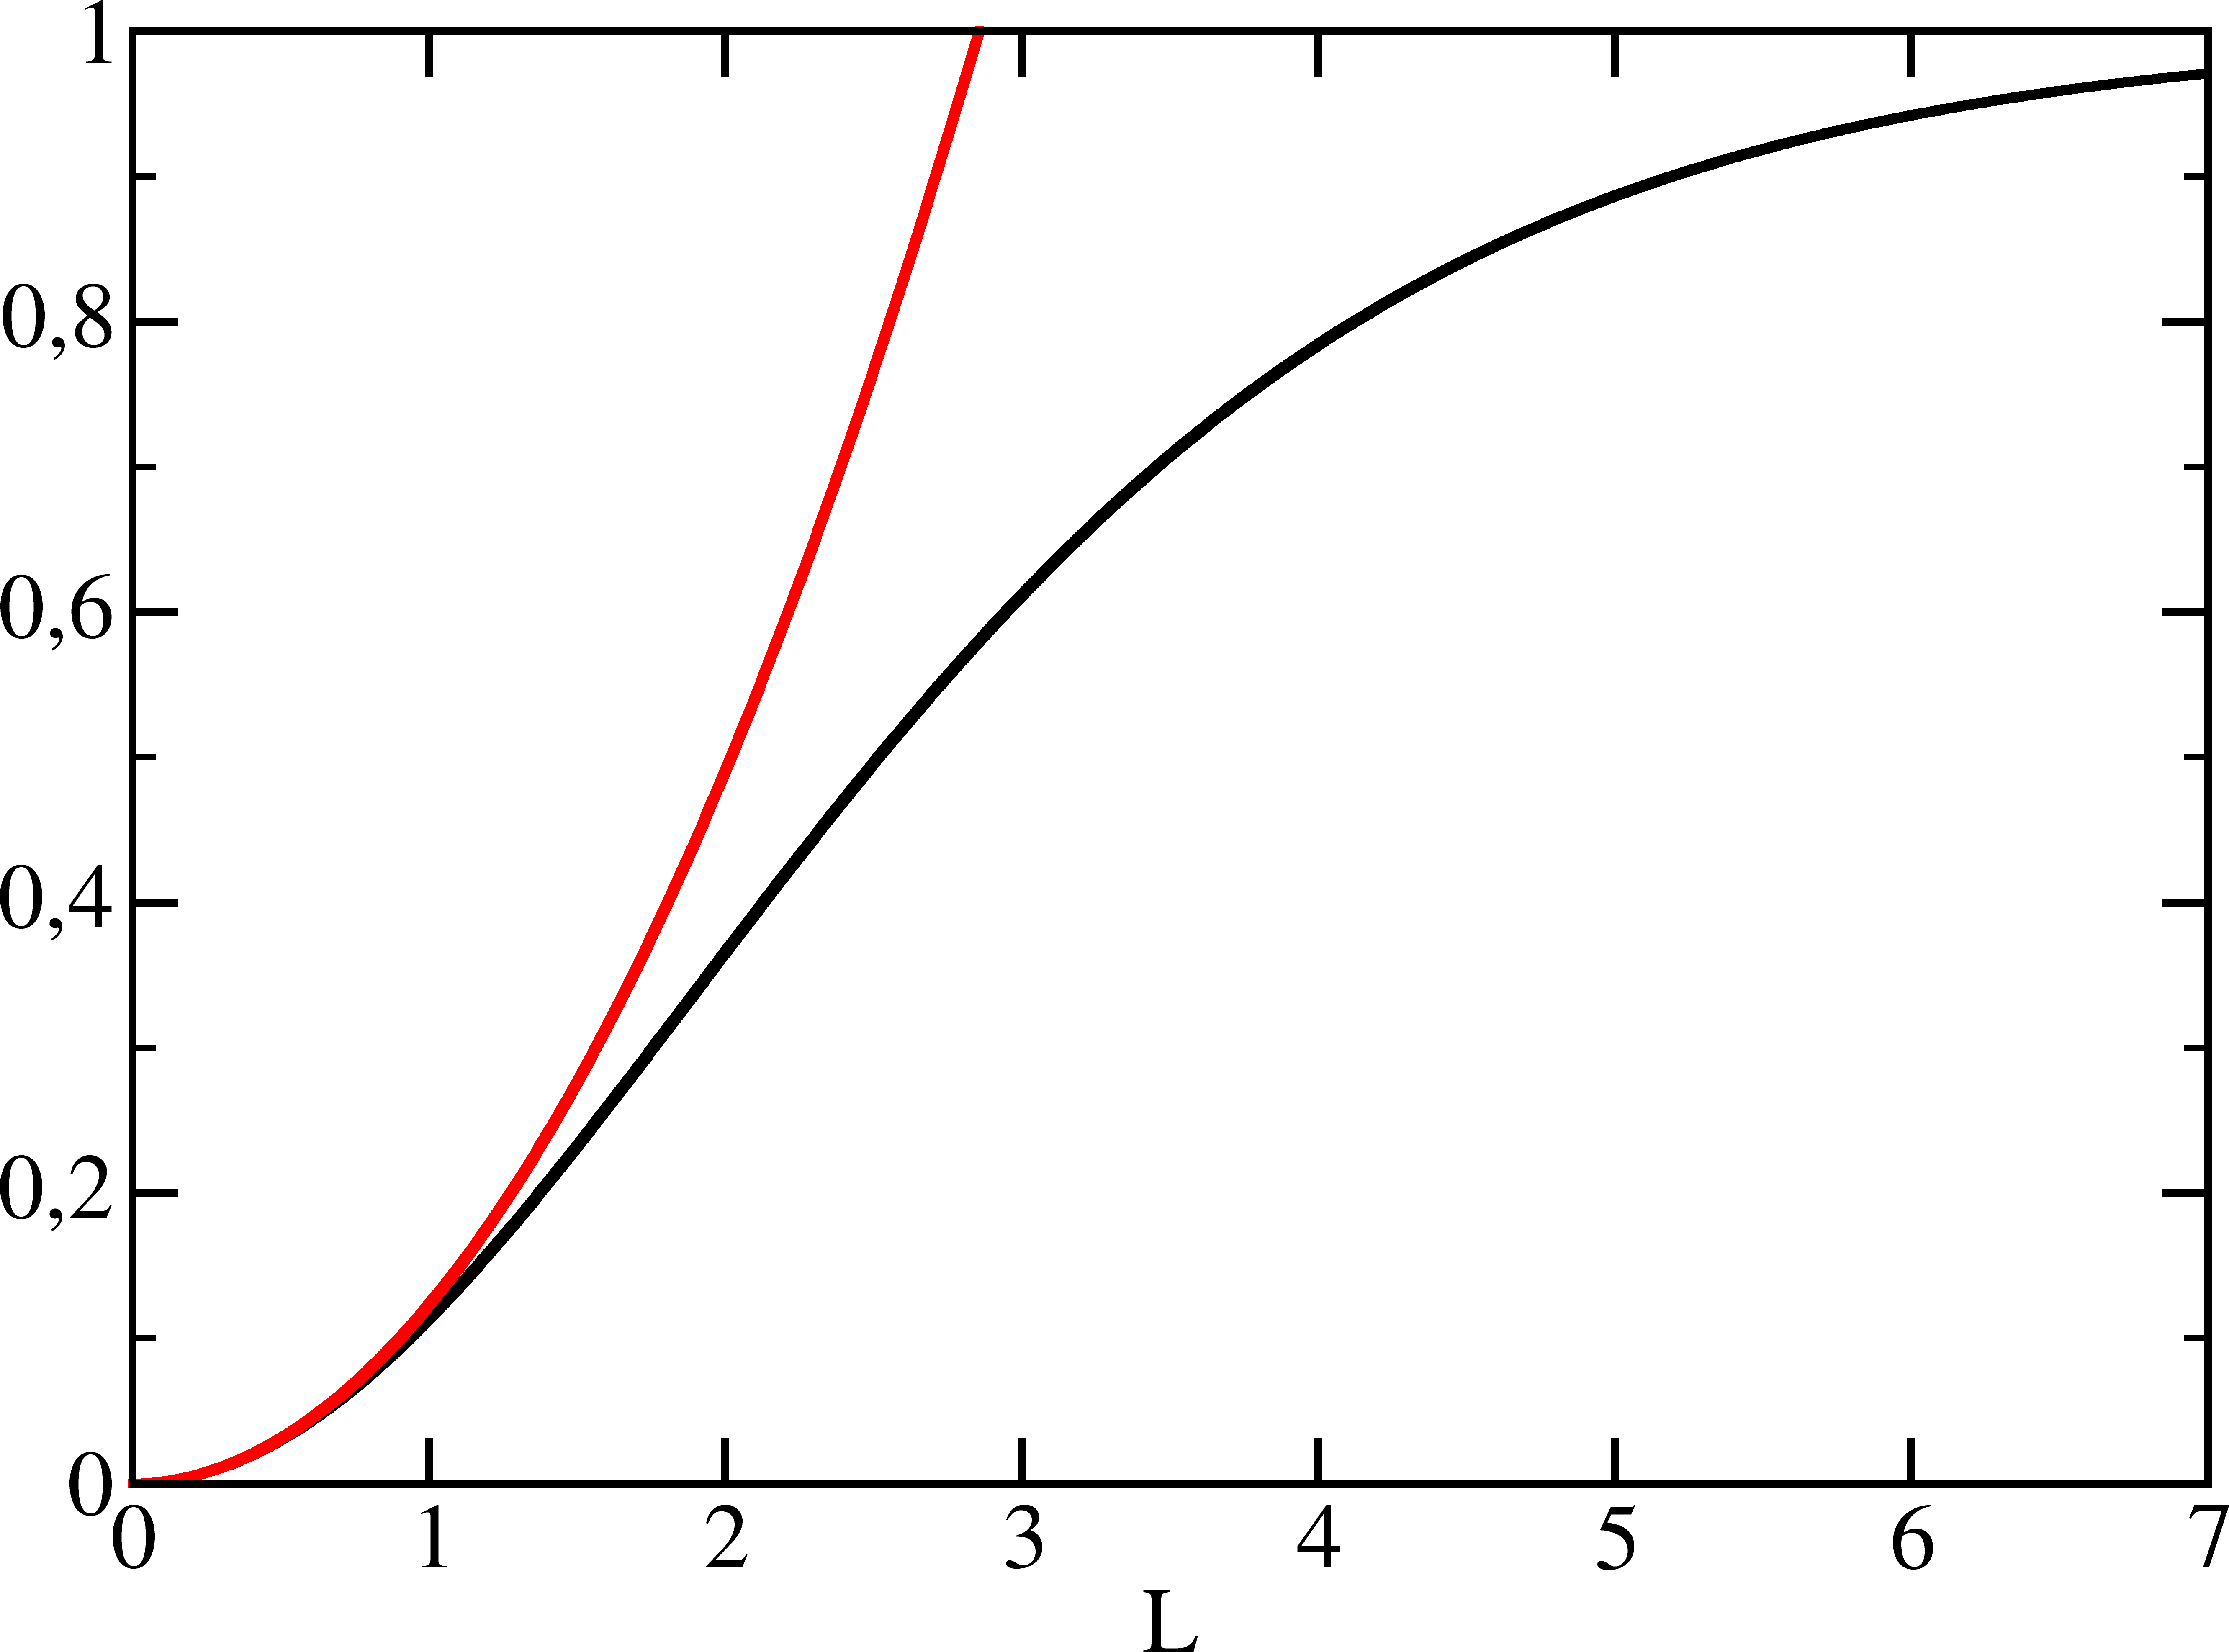
\includegraphics[width=8truecm]{slike/08_shg_depletion.png}
\caption{Izkoristek pretvorbe v frekvenčno podvojeno valovanje. Če privzamemo, da se
intenziteta osnovnega žarka ne zmanjšuje, je odvisnost parabolična (rdeča krivulja), kar 
je dober približek le za majhne intenzitete. Bolj natančen izračun pokaže, da je izkoristek 
pretvorbe sorazmeren s $\tanh^2(\kappa L)$.}
\label{fig:shg2dep}
\end{figure}

Poglejmo še, kaj se zgodi, kadar pogoj ujemanja faz ni izpolnjen in 
 $\Delta k \neq 0$. Takrat dolžino kristala $L$ v izrazu~(\ref{8.11})
pokrajšamo in izkoristek pretvorbe z naraščajočim
$L$ sinusno niha med nič in neko največjo vrednostjo. Tak pojav lahko opazimo, če
uporabimo klinast vzorec, ki se mu debelina spreminja, ali pa če vzorec sučemo 
in na ta način spreminjamo razliko faz. Ta pojav, imenujemo ga Makerjeve 
oscilacije\footnote{P. D. Maker et al., Phys. Rev. Lett. 8, 21 (1962).}, 
uporabljamo za določanje nelinearne susceptibilnost kristalov.\index{Makerjeve oscilacije}

% \begin{remark}
%  Odvisnosti stopnje pretvorbe od razlike valovnih vektorjev pri osnovni
% in podvojeni frekvenci je lahko razumeti s pomočjo slike~(\ref{fig:shg1}). Opazujmo
% prispevka k frekvenčno podvojenem valu, ki nastaneta eden na začetku kristala
% in drugi na koncu. Prispevek z začetka kristala zaradi disperzije na izhodni
% strani ni v fazi s prispevkom s konca. Pri dovolj veliki fazni razliki
% pride do destruktivne interference, ki zmanjšuje moč podvojene svetlobe.
% Razmere so podobne kot pri uklonu na široki reži, kjer prav tako seštevamo
% delna valovanja, ki se jim faza po reži linearno spreminja.
% \begin{figure}[h]
% \centering
% 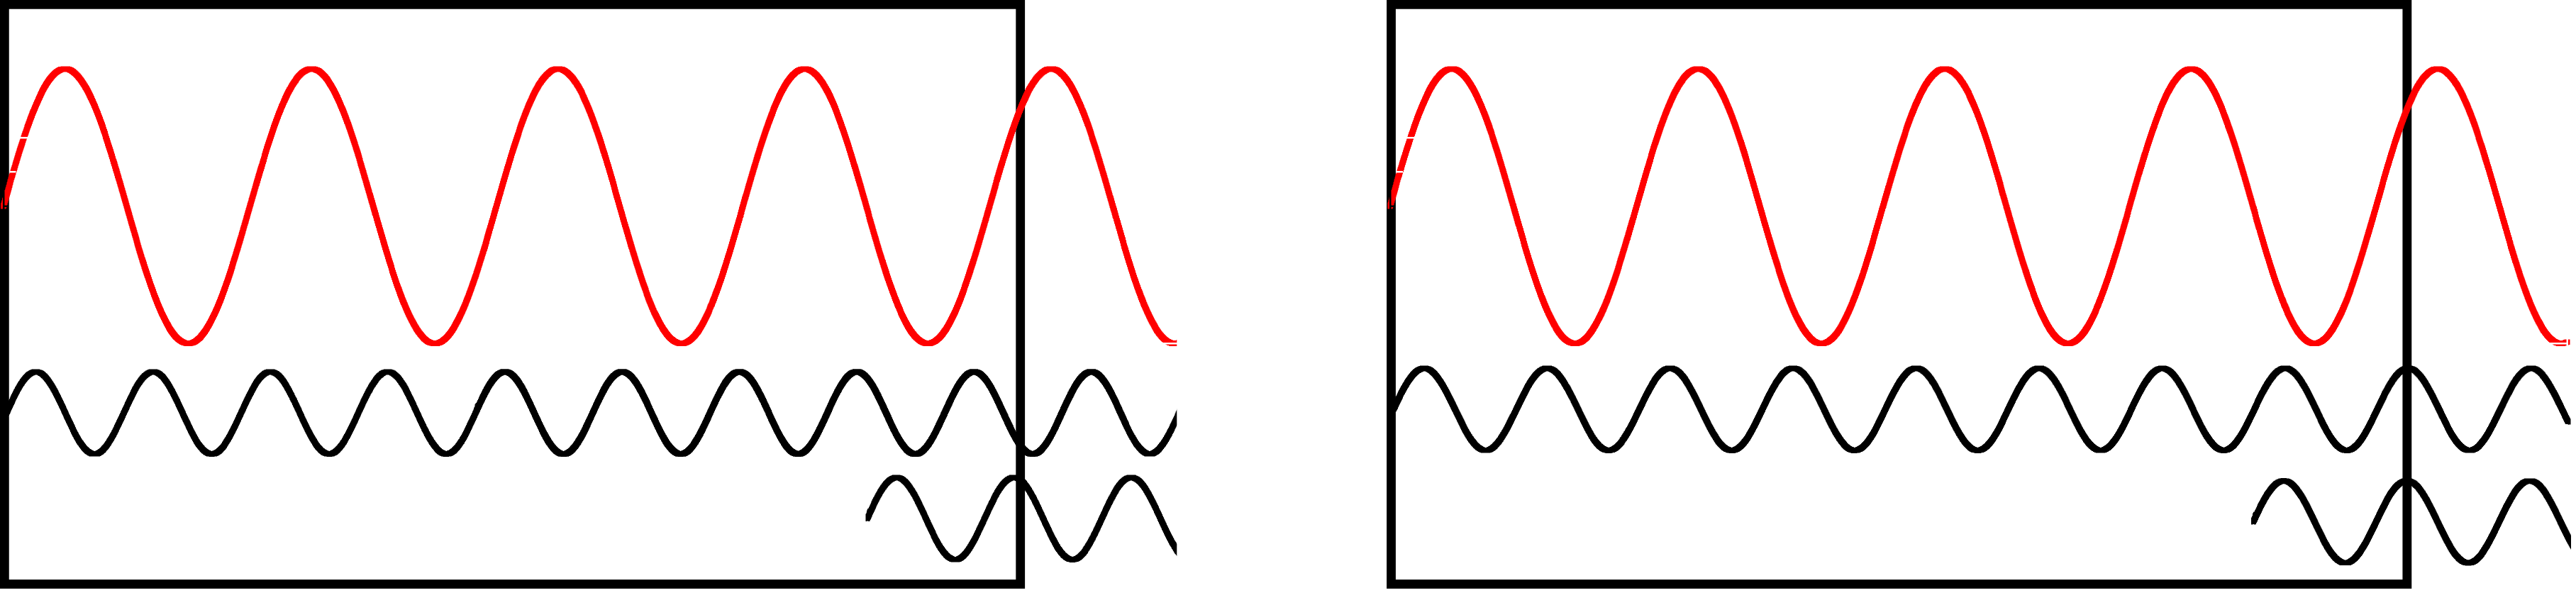
\includegraphics[width=10truecm]{slike/08_shg1.png}
% \caption{Levo: Neujemanje faz privede do destruktivne interference med valovi, ki nastajajo
% v različnih delih nelinearnega sredstva. Desno: V primeru, da se faze ujemajo, se valovanje 
% podvojeni frekvenci ojača.}
% \label{fig:shg1}
% \end{figure}
% \end{remark}

\subsection*{Ujemanje faz}
\index{Ujemanje faz}
Poglejmo, kako lahko dosežemo ujemanje faz, ki je nujno za učinkovito optično
podvajanje frekvenc. Spomnimo se, da je pogoj za ujemanje faz 
\beq
\Delta k = k_3 - k_1 -k_2 = k_3^{2\omega} - k_1^{\omega} -k_2^\omega = 
\frac{2\omega}{c_0} n_3 - \frac{\omega}{c_0} n_1- \frac{\omega}{c_0} n_2 =0.
\eeq
Iz tega sledi pogoj za ujemanje faz
\boxeq{eq:dk0}{
n_1^\omega + n_2^\omega = 2n_3^{2\omega}.
}
Da lahko zadostimo gornjemu pogoju, izkoristimo dvojni lom\index{Dvolomnost} v anizotropnih kristalih
(glej poglavje~\ref{chap:anizotropni}), pri čemer se zaradi enostavnosti omejimo le na optično 
enoosne kristale. Obravnavajmo samo kristale brez absorpcije in z normalno disperzijo, 
to pomeni, da oba lomna količnika naraščata s frekvenco.  

Za razumevanje je najbolj nazoren grafični prikaz (slika~\ref{fig:dk}). 
Podrobneje poglejmo primer s slike (a). Na njem so narisani lomni količniki
\index{Lomni količnik} za pozitivno
anizotropni ($n_e>n_o$) enoosni kristal pri enojni in dvojni
frekvenci v odvisnosti od kota glede na optično os. Rdeča barva nakazuje lomne količnike
pri vpadni frekvenci, modra pa pri podvojeni. Ekscentričnost elipse za 
izredni lomni količnik in frekvenčna disperzija sta zaradi večje nazornosti močno 
pretirani. Opazimo, da je pri nekem kotu $\vartheta$ med smerjo širjenja svetlobe $\mathbf{k}$
in optično osjo $z$ redni lomni količnik pri dvojni frekvenci enak izrednemu količniku pri osnovni
frekvenci. Če torej izberemo izredno polarizacijo vpadnega valovanja (tako, ki leži
v ravnini optične osi in smeri širjenja), bo za podvojeno valovanje z redno
polarizacijo (to je pravokotno na optično os) pri kotu
$\vartheta_m$ izpolnjen pogoj ujemanja faz~(enačba~\ref{eq:dk0}). Zapišimo to še z enačbo.

\begin{figure}[h]
\centering
\def\svgwidth{160truemm} 
\input{slike/08_phasematch.pdf_tex}
\caption{Štirje primeri, pri katerih je izpolnjen pogoj za ujemanje faz. 
(a) Ujemanje faz prvega reda za pozitivno anizotropno snov, (b)
ujemanje faz prvega reda za negativno anizotropno snov ter 
ujemanje faz drugega reda za pozitivno (c) in negativno (d) anizotropno snov.}
\label{fig:dk}
\end{figure}

Lomni količnik za redno polarizirano valovanje pri podvojeni frekvenci mora biti enak lomnemu 
količniku za izredno polarizirano valovanje pri osnovni frekvenci. Pri tem je lomni količnik
za izredno valovanje odvisen od kota
\begin{equation}
\frac{1}{(n_o^{2\omega})^2} = \frac{1}{(n^{\omega}(\vartheta))^2}=
\frac{\cos^{2}\vartheta}{(n_{o}^{\omega})^2}+\frac{\sin^{2}\vartheta}{(n_{e}^{\omega})^2}.
\label{8.12}
\end{equation}
Tako dobimo izraz
\begin{equation}
\cos^{2}\vartheta_m=\frac{(n_o^{2\omega})^{-2}-(n_{e}^{\omega})^{-2}}
{(n_{o}^{\omega})^{-2}-(n_{e}^{\omega})^{-2}},
\label{8.13}
\end{equation}
iz katerega lahko izračunamo kot $\vartheta_m$, pri katerem pride do ujemanja faz.
\begin{definition}
Pokaži, da v primeru negativne anizotropije pogoj za ujemanje faz zapišemo kot
\beq
\cos^{2}\vartheta_m=\frac{(n_o^{\omega})^{-2}-(n_{e}^{2\omega})^{-2}}
{(n_{o}^{2\omega})^{-2}-(n_{e}^{2\omega})^{-2}}.
\label{8.13a}
\eeq
\end{definition}

S slike~(\ref{fig:dk} c in d) lahko razberemo, da obstoja še en primer, pri 
katerem je izpolnjen pogoj za ujemanje faz. Poglejmo primer (c), pri katerem sta v vpadnem
valovanju prisotni obe polarizaciji, redna in izredna, podvojeno valovanje pa
je redno polarizirano. Tedaj mora biti za ujemanje faz vsota rednega in izrednega
lomnega količnika pri osnovni frekvenci enaka dvakratniku rednega lomnega 
količnika pri dvojni frekvenci. Povedano drugače: lomni količnik pri dvojni
frekvenci mora biti enak povprečju rednega in izrednega lomnega količnika
pri osnovni frekvenci. Za praktično uporabo je ta izbira, kadar obstoja,
celo ugodnejša, ker je pri njej kot ujemanja faz bliže $\pi/2$. 
Ujemanje faz je zato manj občutljivo na majhna odstopanja v kotu ali na temperaturne
spremembe lomnih količnikov. Račun kota $\vartheta_m$ za ta primer je
bolj zahteven, saj je treba rešiti enačbo četrte stopnje.

\subsection*{Efektivna susceptibilnost}
\index{Susceptibilnost!nelinearna, efektivna}
Na izhodno moč frekvenčno podvojenega snopa poleg faznega faktorja bistveno vpliva tudi efektivna 
susceptibilnost $\chi_{ef}$, ki jo moramo izračunati za vsak primer posebej. 
V optično enoosnem kristalu
je kriterij ujemanja faz izpolnjen na stožcu okoli optične osi, pri čemer je stožec določen 
z izračunanim kotom $\vartheta_m$ (enačbi~\ref{8.13} in \ref{8.13a}). 
Drugi kot, ki določa smer širjenja v ravnini, ki je pravokotna na optično os, pa 
izberemo tako, da izkoristimo največje komponente nelinearne 
susceptibilnosti. 

Oglejmo si kot primer spet KH$_{2}$PO$_{4}$\index{KDP}, ki je negativno anizotropen 
z vrednostmi $n_o^{\omega} = 1,4942$, 
$n_e^{\omega} = 1,4603$, $n_o^{2\omega} = 1,5129$ in $n_e^{2\omega} = 1,4709$
(slika~\ref{fig:dk}\,b). Valovna dolžina osnovnega snopa naj bo 1064~nm. 
Po podatkih, navedenih zgoraj, dobimo po enačbi~(\ref{8.13a}) za kot ujemanja faz 
$\vartheta_m = 41,25^\circ$. Nelinearna susceptibilnost ima v tetragonalni
simetriji $\bar{4}2m$ od nič različne komponente $\chi_\textrm{xyz}$, $\chi_\textrm{xzy}$
$\chi_\textrm{zxy}$, $\chi_\textrm{zyx}$, $\chi_\textrm{yzx}$ in $\chi_\textrm{yxz}$
(glej tabelo~\ref{table:chi}). 
Zaradi poenostavitve privzamemo, da so njihove vrednosti enake. 

Naj se osnovno in frekvenčno podvojeno valovanje širita 
v smeri $\mathbf{s}$. Pri zapisu vektorja si pomagamo 
s sliko (\ref{fig:chi})
\begin{equation}
\mathbf{s}=(\cos\varphi\sin\vartheta_m,\sin\varphi\sin\vartheta_m,\cos\vartheta_m),
\label{8.14}
\end{equation}
kjer je $\varphi$ kot med osjo $x$ in projekcijo $\mathbf{s}$ na ravnino
$xy$. Naša naloga je poiskati vrednost kota $\varphi$, pri kateri je 
moč frekvenčno podvojenega valovanja največja.
\begin{figure}[h]
\centering
\def\svgwidth{70truemm} 
\input{slike/08_chi.pdf_tex}
\caption{K izračunu efektivne susceptibilnosti. Rdeč vektor označuje
polarizacijo vhodnega valovanja, moder pa polarizacijo frekvenčno podvojenega valovanja.}
\label{fig:chi}
\end{figure}
Iz pogoja za ujemanje faz vidimo, da mora biti vpadna svetloba redno polarizirana, 
izhodna frekvenčno podvojena pa izredno polarizirana. Redna polarizacija je pravokotna na 
os $z$ (optično os) in hkrati pravokotna na smer vektorja $\mathbf{s}$. Zapišemo jo kot
\begin{equation}
\mathbf{e}_o=(\sin\varphi,-\cos\varphi,0).
\label{8.15}
\end{equation}
Izredna polarizacija leži v ravnini, ki jo tvori vektor $\mathbf{s}$ z osjo $z$,
hkrati pa je pravokotna na vektor $\mathbf{s}$, 
tako da jo zapišemo kot 
\begin{equation}
\mathbf{e}_e=(-\cos \varphi \cos \vartheta_m,-\sin \varphi \cos \vartheta_m ,\sin \vartheta_m).
\label{8.15a}
\end{equation}
Spomnimo se, da efektivno susceptibilnost izračunamo kot (enačba~\ref{eq:chicomp})
\beq
\chi_{ef} = \sum_{ijk} \chi_{ijk} e_{3i} e_{1j} e_{2k} = \sum_{ijk} \chi_{ijk} e_{ei} e_{oj} e_{ok}.
\eeq
Krajši račun pokaže, da je zaradi oblike tenzorja nelinearne susceptibilnosti v izbranem 
primeru od nič različna le $z$ komponenta nelinearne polarizacije. Dobimo
\beq
\chi_{ef} = \chi_{\textrm{zxy}} e_{ez} e_{ox} e_{oy} + \chi_{\textrm{zyx}} e_{ez} e_{oy} e_{ox}
\eeq
in
\begin{eqnarray}
P_{\textrm{z}}^{2\omega}&=&- 2\varepsilon_0\, \chi_{\textrm{zxy}}E_{0}^2\cos\varphi\sin\varphi
\sin\vartheta_m \nonumber \\
&=& - \varepsilon_0\, \chi_{\textrm{zxy}}E_{0}^2\sin(2\varphi) \sin\vartheta_m.
\label{8.151}
\end{eqnarray}
Nelinearna polarizacija je največja, kadar je $\varphi=\pi/4$.
Največji efektivni koeficient $\chi_{ef}$, ki nastopa v izrazih za amplitudo in 
moč podvojene svetlobe (enačbi~\ref{8.10} in \ref{8.11}), je torej v izbranem primeru 
\begin{equation}
\chi_{ef}= 
\sin\vartheta_m \chi_{\textrm{zxy}} \approx 0,66\, \chi_{\textrm{zxy}} \approx 0,74~\mathrm{pm/V}.
\label{8.16}
\end{equation}

\begin{definition}
Izračunaj efektivno nelinearno susceptibilnost za frekvenčno podvajanje svetlobe z valovno
dolžino 10~$\mu$m v kristalu telurja s simetrijsko grupo 32 (glej tabelo~\ref{table:chi}). 
Lomni količniki: $n_o^{\omega} = 4,7969$, 
$n_e^{\omega} = 6,2455$, $n_o^{2\omega} = 4,8657$ in $n_e^{2\omega} = 6,3152$.
\end{definition}

\section{Frekvenčno podvajanje Gaussovih snopov}
\index{Optično podvajanje frekvenc}
Doslej smo vpadni in frekvenčno podvojeni snop obravnavali kot ravni valovanji,
ki sta bili razsežni v prečni smeri. Izračunali smo, da v primeru \index{Ujemanje faz}
ujemanja faz ($\Delta k=0$)
moč frekvenčno podvojene svetlobe narašča s kvadratom dolžine poti po nelinearnem
sredstvu. Pretvorba v frekvenčno podvojeno svetlobo je po enačbi~(\ref{8.11}) tem
učinkovitejša, čim večja je gostota svetlobnega toka pri osnovni frekvenci.
Zato v praksi vpadno svetlobo vselej fokusiramo in tako povečamo gostoto toka.  

Poglejmo, kako se enačbe spremenijo, če je vpadni snop pri osnovni 
frekvenci Gaussove oblike\index{Gaussov snop!frekvenčno podvajanje}. 
Rezultat lahko ocenimo, če vzamemo, da je
efektivna dolžina za pretvorbo $L$ kar dolžina grla; izven grla je 
gostota toka znatno manjša kot v grlu, s tem pa tudi izkoristek pretvorbe v 
frekvenčno podvojeni snop.
Dolžina grla je 
\beq
L=2z_{0}=\frac{2n \pi w_{0}^{2}}{\lambda} = \frac{n w_0^2 \omega}{c_0}.
\label{SHGG}
\eeq
Tako je presek vpadnega snopa
\beq
S=\pi w_{0}^{2} = \frac{\pi c_0 L}{n \omega.}
\eeq
Daljše ko je grlo in večja dolžina $L$, na kateri pride do frekvenčnega podvajanja, 
večji je tudi presek snopa $S$ in zato manjša intenziteta svetlobe, kar zmanjša
učinek pretvorbe v frekvenčno podvojeno valovanje.
Vstavimo $S$ v enačbo~(\ref{8.11}), upoštevamo ujemanje faz in dobimo 
\boxeq{8.17}{
\frac{P_{2\omega}}{P_{\omega}}=
\frac{\omega^3 \chi_{ef}^2}{2 \pi n_{2\omega} n_\omega c_0^4\varepsilon_0} P_\omega\, L.
}
Ob optimalnem fokusiranju je torej izkoristek pretvorbe sorazmeren z 
dolžino kristala in ne z njenim kvadratom.

\begin{definition}
Imamo 1~cm dolg kristal KH$_{2}$PO$_{4}$. Valovna dolžina vpadne svetlobe 
je 1,06~$\mu$m, vhodna moč $P_\omega = 10$~kW, efektivna nelinearna susceptibilnost
$\chi_{ef}=7\cdot10^{-13}~$m/V, $\Delta k=0$ in $n=1,5$. Pokaži, da je
faktor pretvorbe v frekvenčno podvojeno svetlobo okoli $20~\%$.

Da je dolžina grla $2z_{0}=1$~cm, mora biti polmer
grla okoli 40~$\mu$m. Gostota svetlobnega toka v kristalu je pri
tem $2\cdot10^{8}$~W/cm$^{2}$, kar je že blizu praga za poškodbe,
predvsem na vstopni ali izstopni površini. Zato je pri podvajanju frekvenc
zelo pomembna odpornost nelinearnega kristala proti poškodbam
zaradi velike gostote svetlobnega toka. To in možnost izpolnitve kriterija ujemanja 
faz sta poglavitna kriterija pri izbiri snovi za frekvenčno podvajanje. 
\end{definition}

\section{{*}Račun podvajanja Gaussovih snopov}
\index{Gaussov snop!frekvenčno podvajanje}
V prejšnjem razdelku smo na hitro grobo ocenili vpliv oblike Gaussovih snopov
na frekvenčno podvajanje. Naredimo zdaj še natančnejši izračun. Vrnimo se k valovni
enačbi~(\ref{8.3}), vpadna snopa naj bosta pri frekvencah
$\omega_{1}$ in $\omega_{2}$, nastajajoč snop pa pri frekvenci
$\omega_{3}=\omega_{1}+\omega_{2}$.
Podobno kot prej naj ima vsako od polj obliko 
\beq
\mathbf{E}_{i}  = \frac{\mathbf{e}_{i}}{2}\left[\tilde{A}_{i}(r,z)\, 
e^{i(k_{i}z-\omega_{i}t)}+\tilde{A}_{i}^{*}(r,z)\, e^{-i(k_{i}z-\omega_{i}t)}\right],
\eeq
pri čemer je $\tilde{A}(r,z)$ zdaj funkcija tako vzdolžne kot tudi prečne koordinate. Privzeli
bomo, da se vzdolž $z$ le počasi spreminja.
Zaradi poenostavljenega zapisa vpeljimo novo spremenljivko 
\beq
\psi_i = \sqrt{\frac{n_i}{\omega_i}}\tilde{A}_i.
\eeq
Tako dobimo nastavek za električno poljsko jakost
\begin{equation}
\mathbf{E}_{i}=\frac{\mathbf{e}_{i}}{2}\sqrt{\frac{\omega_{i}}{n_{i}}}\psi_{i}(r,z)
e^{i(k_{i}z-\omega_{i}t)}+\mbox{ k. k.}
\label{8.18}
\end{equation}
Vstavimo nastavek~(\ref{8.18}) v valovno
enačbo~(\ref{8.3}) in ločimo na levi in desni člene z enako frekvenco.
Zaradi počasnega spreminjanja vzdolž smeri $z$ lahko zanemarimo tudi druge odvode 
$\psi$ po $z$. Tako dobimo sklopljen sistem obosnih enačb 
\begin{eqnarray}
\nabla_{\perp}^{2}\psi_{1}+2ik_{1}\psi_{1}^{\prime} & = & -
\frac{k_{1}}{2}\kappa\psi_{2}^{\ast}\psi_{3}e^{-i\Delta kz}\\
\nabla_{\perp}^{2}\psi_{2}+2ik_{2}\psi_{2}^{\prime} & = & -
\frac{k_{2}}{2}\kappa\psi_{1}^{\ast}\psi_{3}e^{-i\Delta kz}\\
\nabla_{\perp}^{2}\psi_{3}+2ik_{3}\psi_{3}^{\prime} & =
& - \frac{k_{3}}{2}\kappa\psi_{1}\psi_{2}e^{i\Delta kz}
\label{SHGGauss_3}
\end{eqnarray}
s pripadajočim sistemom konjugiranih enačb. Pri tem je 
\begin{equation}
\kappa=\frac{\chi_{ef}}{c_0} \sqrt{\frac{\omega_{1}\omega_{2}\omega_{3}}{n_{1}n_{2}n_{3}}}.
\label{8.20}
\end{equation}
S črtico smo označili odvajanje po $z$. Gornji sistem enačb je očitno
posplošitev sistema enačb~(\ref{eq:nlAz} do \ref{eq:nlA3}) za primer, ko je valovanje odvisno
tudi od prečne koordinate. Reševanje tega nelinearnega sistema parcialnih
diferencialnih enačb je v splošnem zelo zapleteno.

Poglejmo le najenostavnejši primer frekvenčnega podvajanja, ko je 
$\omega_{3}=2\omega_{1}=2\omega$.
Vpadna snopa naj bosta enaka in Gaussove oblike~(enačba~\ref{eq:gaussov-snop}), 
njuna amplituda pa naj bo enaka $A_1$
\begin{equation}
\psi_{1} = \psi_2 = A_{1}\frac{1}{1+iz/z_1}
\exp\left(-\frac{r^{2}}{w_1^{2}(z)}+\frac{ik_1r^{2}}{2R_1(z)}\right).
\label{8.21}
\end{equation}
Privzemimo še, da je izpolnjen pogoj za ujemanje faz\index{Ujemanje faz}, $\Delta k=0$,
in da je $\psi_{3}$ dovolj majhen, da nam zmanjševanja $\psi_{1}$
ni treba upoštevati. Tudi za podvojeni snop privzemimo Gaussovo 
obliko, njegova amplituda $A_3$ pa naj le počasi narašča. Zapišemo ga kot
\begin{equation}
\psi_{3}=A_{3}(z)\psi_{3H}(z,r)=A_{3}(z)\frac{1}{1+iz/z_{3}}
\exp\left(-\frac{r^{2}}{w_{3}^{2}(z)}+\frac{ik_{3}r^{2}}{2R_{3}(z)}\right),
\label{8.22}
\end{equation}
pri čemer $\psi_{3H}$ reši homogeno obosno valovno 
enačbo~(\ref{eq:obosna-valovna-enacba})\index{Obosna valovna enačba}. Ko izraza za $\psi_{1}$
in $\psi_{3}$ vstavimo v tretjo enačbo sistema sklopljenih enačb (\ref{SHGGauss_3}),
ostane na levi le člen oblike $2ik_{3}A_{3}^{\prime}(z)\psi_{3H}$. Tako dobimo pogoj
\begin{equation}
A_{3}^{\prime}(z)\frac{1}{1+iz/z_3}\exp\left(-\frac{r^{2}}{w_{3}^{2}(z)}+\frac{ik_{3}r^{2}}
{2R_{3}(z)}\right)=
\frac{i\kappa}{4}A_{1}^{2}\frac{1}{(1+iz/z_{1})^{2}}\exp\left(-\frac{2r^{2}}
{w_{1}^{2}(z)}+\frac{ik_{1}r^{2}}{R_{1}(z)}\right).
\label{8.23}
\end{equation}
Poiščimo rešitev te enačbe v obliki, za katero velja $w_{30}^{2}=w_{10}^{2}/2$. Tedaj je 
\beq
z_{3}=\frac{k_{3}w_{30}^{2}}{2}=\frac{2k_{1}w_{10}^{2}}{4}=z_{1}
\eeq
in je tudi $w_{3}^{2}(z)=w_{1}^{2}(z)/2$. Poleg tega je $R_{3}(z)=R_{1}(z)$
in lahko na obeh straneh pokrajšamo eksponentna faktorja. Ostane 
\begin{equation}
A_{3}^{\prime}(z)=\frac{i\kappa}{4}A_{1}^{2}\frac{1}{1+iz/z_1}.
\label{8.24}
\end{equation}
Gornjo enačbo seveda brez težav integriramo. Naj bo grlo vpadnega
snopa ravno na sredini nelinearnega sredstva, tako da integriramo
od $-L/2$ do $L/2$
\begin{eqnarray}
A_{3}(L) & = & \frac{i\kappa}{4}A_{1}^{2}\int_{-L/2}^{L/2}\frac{dz}{1+iz/z_1} 
  = \frac{\kappa}{4}A_{1}^{2}z_{1}\ln\frac{1+i\frac{L}{2z_{1}}}{1-i\frac{L}{2z_{1}}}= \nonumber \\
 & = & \frac{\kappa}{2}A_{1}^{2}z_{1}\arctan\frac{L}{2z_{1}}\;.
\end{eqnarray}
Moč Gaussovega snopa je
\begin{equation}
P_{i}=\pi w_{i0}^{2} \frac{1}{2}c_0 n_i \epsilon_{0}E_{i0}^{2}=
\frac{\pi}{2}w_{i0}^{2}\varepsilon_0 c_0 \omega_{i} A_{i}^{2},
\label{8.26}
\end{equation}
tako da je izkoristek pri frekvenčnem podvajanju Gaussovega snopa 
\begin{equation}
\frac{P_{2\omega}}{P_{\omega}}=\frac{A_3^2}{A_1^2} = 
\frac{\chi_{ef}^2 \omega^3 P_\omega z_1}{2 \pi c_0^4 \varepsilon_0 n_1 n_3} 
\arctan^2 \left( \frac{L}{2z_1}\right)
= \frac{\chi_{ef}^2 \omega^3 P_\omega}{2 \pi c_0^4 \varepsilon_0 n_1 n_3} \frac{L}{2}
\arctan^2 \left( \frac{L}{2z_1}\right) \frac{1}{L/2z_1}.
\label{8.27}
\end{equation}
Funkcija $(\arctan^{2}x)/x$ zavzame največjo vrednost 0,64 pri $x =L/2z_1=1,39$.
Pri dani dolžini nelinearnega sredstva $L$ je torej 
izkoristek največji, kadar je $z_{1}=0,36\,L$, kar je malo manj kot pri
preprosti oceni $z_{1}=0,5\,L$ (enačba~\ref{SHGG}). Največji izkoristek
frekvenčnega podvajanja Gaussovih snopov je tako
\begin{equation}
\frac{P_{2\omega}}{P_{\omega}}
= 0,32 \frac{\chi_{ef}^2 \omega^3 }{2 \pi c_0^4 \varepsilon_0 n_1 n_3} P_\omega L.
\label{8.28}
\end{equation}
To je malo manj od preproste ocene, ki smo jo naredili v prejšnjem razdelku (enačba~\ref{8.17}),
v obeh primerih pa izkoristek narašča linearno z dolžino kristala.

\section{Optično parametrično ojačevanje}
\index{Optično parametrično ojačevanje}
\index{Parametrično ojačevanje|see{Optično parametrično ojačevanje}}

Oglejmo si še en zelo uporaben primer mešanja treh valovanj, 
ki ga opisujejo enačbe (\ref{eq:nlAz}) do (\ref{eq:nlA3}). Gre za
optično parametrično ojačevanje, pri katerem nelinearne optične pojave
izkoristimo za ojačevanje optičnih signalov. Imejmo vhodni
signal pri frekvenci $\omega_{1}$, ki ga želimo ojačati, in močno črpalno valovanje
pri frekvenci $\omega_{3}>\omega_{1}$. Zaradi nelinearnosti v snovi se 
intenziteta valovanja pri $\omega_{1}$ povečuje, 
intenziteta valovanja pri $\omega_{3}$ zmanjšuje, hkrati pa zaradi
ohranitve energije nastaja dodatno valovanje pri razliki frekvenc
$\omega_{2}=\omega_{3}-\omega_{1}$. Proces parametričnega ojačevanja 
si torej lahko predstavljamo kot pretvorbo enega fotona pri frekvenci 
$\omega_{3}$ v dva fotona pri $\omega_{1}$ in $\omega_{2}$.
Parametrično ojačevanje pogosto uporabljamo za ojačevanje šibkih signalov 
v infrardečem območju.
\begin{figure}[h]
\centering
\def\svgwidth{100truemm} 
\input{slike/08_opa.pdf_tex}
\caption{Shematski prikaz nastanka valovanj pri optičnem parametričnem ojačevanju}
\label{fig:opa2}
\end{figure}

Izhajamo iz splošnih enačb za nelinearne optične pojave drugega reda (enačbe~\ref{eq:nlAz} do
\ref{eq:nlA3}). 
\begin{eqnarray}
\frac{dA_{3}}{dz} &=& \frac{i\omega_{3}\chi_{ef}}{4c_0 n_3} A_{1}\, A_{2}\, e^{-i\Delta kz}\\
\frac{dA_{2}}{dz} &=&\frac{i\omega_{2}\chi_{ef}}{4c_0 n_2} A_{1}^*\, A_{3}\, e^{i\Delta kz}\\
\frac{dA_{1}}{dz} &=&\frac{i\omega_{1}\chi_{ef}}{4c_0 n_1} A_{2}^*\, A_{3}\, e^{i\Delta kz}.
\label{eq:opaA}
\end{eqnarray}
Privzemimo, da je črpalno valovanje vselej dosti močnejše od drugih dveh
($A_{3}\gg A_{1}$, $A_{2}$) in njegova jakost približno konstantna $A_3 = A_{30}$.
Poskrbimo še, da je izpolnjen pogoj za ujemanje faz, $\Delta k=0$, 
začetna pogoja pa zapišemo kot $A_{1}(z=0)=A_{10}$ in $A_{2}(z=0)=0$. Ko vse to upoštevamo,
dobimo dve sklopljeni enačbi
\begin{eqnarray}
\frac{dA_{1}}{dz} &=& \frac{i\omega_{1}\chi_{ef}}{4c_0 n_1} A_{2}^*\, A_{30}\label{eq:opaA1} 
\qquad \mathrm{in} \\
\frac{dA_{2}^*}{dz} &=& -\frac{i\omega_{2}\chi_{ef}}{4c_0 n_2} A_{1}\, A_{30}^*.
\label{eq:opaA2}
\end{eqnarray}
Enačbi lahko rešimo, tako da prvo odvajamo po $z$ in vanjo vstavimo drugo enačbo.
Dobimo
\beq
\frac{d^2 A_1}{d z^2} = \frac{\omega_1 \omega_2 \chi_{ef}^2|A_{30}|^2}
{16 c_0^2 n_1 n_2} A_1 = \kappa^2 A_1
\eeq
in podobno za $A_2$
\beq
\frac{d^2 A_2}{d z^2} = \frac{\omega_1 \omega_2 \chi_{ef}^2|A_{30}|^2}
{16 c_0^2 n_1 n_2} A_2 = \kappa^2 A_2.
\eeq
Ob upoštevanju začetnih pogojev dobimo rešitev za naraščanje amplitude signalnega žarka
z začetno amplitudo $A_{10}$
\boxeq{eq:opa}{
A_1 = A_{10} \cosh (\kappa L).
}
Hkrati z njim narašča tudi amplituda dodatnega nedejavnega ({\it idle}) žarka, ki nastane
med procesom ojačanja
\boxeq{eq:opan}{
A_2 = A_{20} \sinh (\kappa L).
}
V gornjih enačbah je $L$ dolžina nelinearnega sredstva, 
\beq
\kappa^2 = \frac{\omega_1 \omega_2 \chi_{ef}^2|A_{30}|^2}
{16 c_0^2 n_1 n_2} 
\label{opakapa}
\eeq
in
\beq
A_{20} = i \sqrt{\frac{\omega_2 n_1}{\omega_1 n_2}} A_{10}.
\label{opakapaA}
\eeq
Na začetku intenziteti obeh valovanj naraščata približno eksponentno na račun črpalnega
valovanja. Ko postane njuna intenziteta znatna in se začne $A_3$ zmanjševati, je treba to seveda
tudi upoštevati pri izračunu. V tem primeru je treba rešiti bolj zahteven sistem treh 
sklopljenih enačb, podobno~\textendash~a še bolj zapleteno~\textendash~kot v nalogi~(\ref{deplet}).

\begin{definition}
Pokaži, da sta izraza za amplitudi polji $A_1$ in $A_2$ (enačbi~\ref{eq:opa} in~\ref{eq:opan})
rešitvi sklopljenih enačb~(\ref{eq:opaA1}) in (\ref{eq:opaA2}) ob parametrih $A_{20}$ in $\kappa$, kot sta zapisana v enačbah~(\ref{opakapa}) in (\ref{opakapaA}).
\end{definition}

Do zdaj smo vedno privzeli, da je izpolnjen pogoj ujemanja faz \index{Ujemanje faz}
in $\Delta k=k_{3}-k_{1}-k_{2}=0$. 
Ta pogoj lahko izpolnimo na enak način kot pri podvajanju frekvence: v dvolomnem kristalu 
izberemo ustrezno smer glede na optično os in ustrezne polarizacije, 
tako da velja $\omega_{3}n_{3}=\omega_{1}n_{1}+\omega_{2}n_{2}$.

Lahko na primer vzamemo izredno polarizacijo za črpalno valovanje
in redni polarizaciji za obe ojačevani valovanji, podobno kot pri
podvajanju frekvence. Tedaj mora biti izpolnjen naslednji pogoj 
\begin{equation}
\left[\left(\frac{\cos\vartheta_{m}}{n_{o}^{\omega_{3}}}\right)^{2}
+\left(\frac{\sin\vartheta_{m}}{n_{e}^{\omega_{3}}}\right)^{2}\right]^{-1/2}=
\frac{\omega_{1}}{\omega_{3}}n_{o}^{\omega_{1}}+\frac{\omega_{2}}{\omega_{3}}n_{o}^{\omega_{2}}.
\label{8.34}
\end{equation}

\begin{figure}[h]
\centering
\def\svgwidth{90truemm} 
\input{slike/08_opagraf.pdf_tex}
\caption{Normirani intenziteti ojačanega žarka in dodatnega žarka, ki nastane zaradi ohranitve
energije. Naraščajoči funkciji sta seveda samo približek, ki velja, dokler je ojačanje majhno in 
se intenziteta črpalnega žarka ne zmanjšuje znantno.}
\label{fig:opagraf}
\end{figure}

\begin{definition}
Obravnavali smo optično parametrično ojačevanje, ko je bil izpolnjen kriterij za ujemanje faz. 
Pokaži, v primeru neujemanja faz $\Delta k \neq 0$ amplitudi ojačevanega in dodatnega 
žarka naraščata kot \index{Neujemanje faz}
\beq
A_1 = A_{10} \left( \cosh(\kappa z) - \frac{i \Delta kz}{2 \kappa} \sinh (\kappa z) 
\right) e^{\frac{i \Delta kz}{2}}\\
A_2 = A_{20} \sinh(\kappa z) e^{\frac{i \Delta k}{2}},
\eeq
pri čemer sta
\beq
\kappa^2 = \frac{\omega_1 \omega_2 \chi_{ef}^2|A_{30}|^2}
{16 c_0^2 n_1 n_2} - \frac{\Delta k^2}{4} \quad \mathrm{in} \quad
A_{20} = i \sqrt{\frac{\omega_2 n_1}{\omega_1 n_2}} \sqrt{1 + \frac{\Delta k^2}{4 \kappa^2}}
~A_{10}.
\eeq
Hitro uvidimo, da so gornje enačbe v limitnem primeru $\Delta k = 0$ enake 
enačbam~(\ref{eq:opa}, \ref{eq:opan} in \ref{opakapa}).
\end{definition}

Za konec ocenimo koeficient ojačanja v nelinearnem kristalu 
LiNbO$_{3}$\index{LiNbO$_3$}, v katerem želimo
ojačati svetlobo z valovno dolžino $\lambda = 1~\mu$m. Črpajmo z laserjem z valovno dolžino 
okoli 500~nm in gostoto svetlobnega toka 5~MW/cm$^{2}$. Lomni količnik snovi je 
$n = 2,2$, $\chi_{ef} = 5$~pm/V. Vstavimo podatke v enačbo~(\ref{opakapa}) in dobimo vrednost
$\kappa \sim 0,15$/cm. Faktor ojačanja vpadne intenzitete svetlobe v 1~cm dolgem kristalu je 
tako le približno $2~\%$. 

\subsection*{Optični parametrični oscilator (OPO)}
\index{Optični parametrični oscilator}
Gornji izračun kaže, da optično parametrično ojačevanje pri prehodu skozi kristal ni prav veliko
kljub dokaj močnemu črpalnemu žarku. Zato je smiselno, da svetloba skozi ojačevalno 
sredstvo preide večkrat in se postopoma ojačuje. To naredimo tako, 
da optično ojačevalno sredstvo zapremo v optični 
resonator\index{Resonator!parametrični oscilator}
in signal se ob vsakem obhodu ojača. Dobimo t.\,i.\,optični parametrični oscilator. 
\begin{figure}[h]
\centering
\def\svgwidth{100truemm} 
\input{slike/08_opo.pdf_tex}
\caption{Shematski prikaz tipičnega optičnega parametričnega oscilatorja. Ojačevalno sredstvo
zapremo med resonatorja, da se signalni žarek ($\omega_1$) ob vsakem preletu ojači.}
\label{fig:opo}
\end{figure}

V optičnemu resonatorju je odbojnost zrcal za črpalni žarek ($\omega_3$) zelo majhna, 
odbojnost za ojačani žarek pa blizu ena. Valovanje pri $\omega_1$,
ki se v parametričnem oscilatorju ojačuje, nastane spontano, prav tako valovanje pri 
$\omega_2 = \omega_3 -\omega_1$. Njuni frekvenci sta dodatno določeni s pogojem za 
ujemanje faz $ k_3 - k_1 - k_2 = 0$, 
hkrati pa mora ojačevano nihanje sovpadati z lastnim nihanjem resonatorja. 
S sukanjem ojačevalnega kristala lahko na ta način spreminjamo
ojačano frekvenco in dobimo nastavljiv izvor svetlobe, navadno infrardeče. 

Za delovanje oscilatorja biti jakost črpalnega žarka tako velika, da je parametrično 
ojačevanje na obhod večje od izgub. Izračunajmo za primer prag simetričnega oscilatorja. Signal z močjo 
$P_0$ se ob prehodu skozi ojačevalno sredstvo ojača (enačba~\ref{eq:opa}) in dobimo
\beq
P_1 = P_0 \cosh^2 (\kappa L),
\eeq
hkrati pa se zaradi delno prepustnih zrcal z odbojnostjo $R$ intenziteta žarka zmanjšuje. 
Pri tem ne pozabimo, da je pogoj ujemanja faz izpolnjen le v eni smeri in se svetloba
ojačuje le enkrat na celoten obhod. Ob preletu v drugo smer je namreč $\Delta k \neq 0$ in žarek se ne ojačuje.
Moč žarka po obhodu $P_2$ je enaka začetni moči $P_0$, saj je pri pragu ojačanje ravno enako izgubam 
\beq
P_2 = R^2 P_1 = R^2 P_0 \cosh^2 (\kappa L) = P_0
\eeq
oziroma
\beq
R^2 \cosh^2 (\kappa L) =1.
\eeq
Iz gornjega pogoja določimo parameter $\kappa$, po enačbi~(\ref{opakapa}) pa mejno 
amplitudo in intenziteto črpalnega žarka. Nadaljujmo še prejšnji primer ojačanja 
svetlobe v 1~cm dolgem kristalu LiNbO$_{3}$.
Če je odbojnost zrcal $R=0,9$ in prečni presek žarka $10~\mu$m$^2$, je moč 
praga $P_{\omega_3} = 5$~W.

\begin{remark}
Optični parametrični oscilator torej oddaja svetlobo, podobno kot laser. Tudi sicer
sta si do neke mere podobna: oba sistema potrebujeta močen črpalni mehanizem, oba sistema
sta sestavljena iz resonatorja, v katerem se žarek velikokrat odbije in postopoma ojača,
in oba oddajata koherentno svetlobo pri točno določeni valovni dolžini. Vendar
je med parametričnim oscilatorjem in laserjem velika razlika. Pri laserju pride do
ojačanja svetlobe zaradi obrnjene zasedenosti stanj, pri oscilatorju pa 
zaradi nelinearnega optičnega pojava. Ker pri oscilatorju energija ni shranjena v
snovi, ampak se ojača sproti, je zelo pomembno, da sunek črpalnega laserja vpade
na kristal istočasno kot ojačevan žarek. Velika prednost oscilatorjev pred laserji 
je zvezno nastavljiva frekvenca delovanja v zelo širokem frekvenčnem območju.  
\end{remark}

\section{Optično usmerjanje in teraherčno valovanje}
\index{Optično usmerjanje}
\index{Teraherčno valovanje}
Ko smo obravnavali nelinearne optične pojave drugega reda, smo zapisali
različne frekvence, ki so vsebovane v izhodnem signalu (slika~\ref{fig:nl2}). Eno izmed
izhodnih valovanj ima tudi frekvenco enako nič, kar pomeni, da je to statično električno polje. Iz analogije
z elektronskimi vezji, kjer izmenično napetost z usmernikom spremenimo v enosmerno napetost, 
pojav imenujemo optično usmerjanje, saj iz svetlobnega valovanja nastane statično polje. Tako statično 
polje navadno ni veliko, saj sunek svetlobe z vršno močjo nekaj MW tipično povzroči 
nekaj deset mV napetosti v smeri prečno na smer potovanja svetlobe. 

\begin{definition}
Pokaži, da je napetost, ki se pojavi pri optičnem usmerjanju, približno enaka
\beq
U = \frac{\chi P_0}{n^3 \varepsilon_0 c_0 a},
\eeq
pri čemer je $P_0$ moč vpadne svetlobe, $n$ lomni količnik snovi in $a$ širina kristala.
Namig: nelinearen kristal obravnavaj kot ploščati kondenzator. Oceni še napetost, če je
$\chi = 3$~pV/m, $P_0 = 1$~MW, $n = 2,2$ in $a = 5$~mm. 
\end{definition}

Precej bolj uporaben je pojav, ko na nelinearen kristal posvetimo z ultrakratkimi 
sunki svetlobe, tipično okoli ps ali krajšimi. Spomnimo se, da je povsem monokromatsko valovanje
lahko samo tako, ki ima neskončnen koherenčni čas in je časovno neomejeno 
(\ref{eq:spektralna-sirina-zveza}). 
Če je valovanje časovno omejeno, je njegov spekter končno širok, pri čemer imajo krajši 
sunki svetlobe širši spekter valovanja. Ko z ultrakratkim sunkom osvetlimo optično 
nelinearen kristal, v kristal vstopajo vse frekvence z danega intervala $\omega \pm \Delta \omega$.
Optično usmerjanje ni več popolno, saj se frekvence ne odštejejo povsem, ampak se 
namesto statičnega polja pojavi valovanje pri frekvencah, ki so podobne širini spektra. Ocenimo jih. 

\begin{figure}[h]
\centering
\def\svgwidth{90truemm} 
\input{slike/08_THz.pdf_tex}
\caption{Shematski prikaz nastanka teraherčnega valovanja v optično nelinearnem sredstvu}
\label{fig:THz}
\end{figure}

S sunkom, ki je dolg 1~ps, tako dobimo
\beq
\Delta \omega = \frac{1}{\tau} = \frac{1}{10^{-12}~\mathrm{Hz}} = 1~\mathrm{THz}.
\eeq
Valovanje, ki nastane pri takem kvazi optičnem usmerjanju, ima torej frekvence v teraherčnem
področju in naredili smo izvor teraherčnega valovanja. Teraherčno valovanje, to je 
elektromagnetno valovanje s frekvencami v območju od 0,3 do 3~THz oziroma z valovnimi dolžinami 
med 0,1 in 1~mm, se uporablja za neinvazivno slikanje in preiskave tkiv in materialov. Kristali, ki 
se najpogosteje uporabljajo za nastanek teraherčnega valovanja, so ZnTe, GaP, GaSe in GaAs.

\section{Nelinearni pojavi tretjega reda}
\index{Nelinearna optika!tretjega reda}
Doslej smo obravnavali najnižji red nelinearnosti, katerega glavni
učinek je mešanje treh frekvenc, na primer podvajanje frekvence ali
parametrično ojačevanje. Ti pojavi so možni le v kristalih brez centra
inverzije. Naslednji člen razvoja nelinearne polarizacije po električnem
polju obstaja v vsaki snovi. V njem nastopa polje v tretji potenci
\boxeq{eq:nl3P}{
\mathbf{P}_{\mathrm{NL,3}}= \epsilon_{0}\chi^{(3)}\vdots \mathbin 
\mathbf{E}\mathbin \mathbf{E}\mathbin\mathbf{E}
}
oziroma izpisano po komponentah
\beq
\left(\mathbf{P}_{\mathrm{NL,3}}\right)_i= \epsilon_{0}\chi^{(3)}_{ijkl} \,E_j \,E_k\, E_l.
\eeq
Pri tem je $\chi^{(3)}$ tenzor četrtega ranga, tipična velikost pa je okoli 
$10^{-22}$~m$^2$/V$^2$. V splošnem ima 81 različnih neodvisnih komponent, to
število pa se lahko zelo zmanjša zaradi simetrije snovi. V izotropni snovi je tako
21 neničelnih elementov, od katerih so le trije neodvisni. 

Če vsebuje vpadno polje le eno frekvenco, se zaradi nelinearnosti tretjega
reda pojavi polarizacija pri 3$\omega$ in $\omega$. Pri dveh vpadnih
frekvencah $\omega_{1}$ in $\omega_{2}$ so možne kombinacije $2\omega_{1}\pm\omega_{2}$
in $\omega_{1}\pm2\omega_{2}$, pri treh vpadnih frekvencah pa vse
možne vsote in razlike frekvenc, to so $\omega_1$, $\omega_2$, $\omega_3$, 
$3\omega_1$, $3 \omega_2$, $3\omega_3$, 
$\omega_1 + \omega_2 + \omega_3$, $\omega_1 + \omega_2 - \omega_3$, 
$\omega_1 - \omega_2 + \omega_3$, $- \omega_1 + \omega_2 + \omega_3$, 
$2 \omega_1\pm\omega_2$, $2 \omega_1\pm\omega_3$, $2 \omega_2\pm\omega_1$,
$2 \omega_2\pm\omega_3$, $2 \omega_3\pm\omega_1$, $2 \omega_3\pm\omega_2$.
Možnosti je torej precej več kot pri nelinearnosti drugega reda in računi so zato 
v splošnem precej zapletenejši.

Obravnava nastanka valovanja pri
kombinaciji frekvenc je zelo podobna obravnavi podvajanja frekvence in parametričnemu
ojačevanju. V enačbah za nastanek novega valovanja ali ojačevanje
katerega od vpadnih snopov spet nastopi fazni faktor, ki vsebuje razliko
vseh valovnih vektorjev $\Delta{\bf k}$. Da bo nastajanje novega
valovanja znatno, mora biti $\Delta kL\simeq0$, spet mora biti torej
izpolnjen pogoj ujemanja faz. Ker v tem primeru nastopajo v splošnem štirje
valovni vektorji, je seveda tudi pri izbiri geometrije in polarizacij
za ujemanje faz precej več možnosti.\index{Ujemanje faz}

Vrnimo se k najpreprostejšemu primeru, ko ima vpadno valovanje le eno 
frekvenco. Takrat se pojavi valovanje pri potrojeni frekvenci, pa tudi
pri frekvenci, ki je enaka vpadni. Pojavi se torej polarizacija pri 
vpadni frekvenci, ki spremeni obnašanje osnovnega žarka, in žarek vpliva sam nase.
Ti pojavi, ki jih poimenujemo s predpono {\it samo-}, kot na primer samozbiranje, so
značilni za nelinearne pojave tretjega reda\index{Samozbiranje}. 

\section{Optični Kerrov pojav}
\index{Optični Kerrov pojav|see Kerrov pojav!optični}
\index{Kerrov pojav!optični}
Naj valovanje vpada na nelinearno snov, za katero velja $\chi^{(2)} = 0$.
Polarizacija je potem enaka vsoti linearnega in nelinearnega dela tretjega reda 
(enačba~\ref{8.1})\index{Električna polarizacija}
\beq
\mathbf{P}=
\epsilon_{0} \chi^{(1)}\cdot \mathbf{E}+
\epsilon_{0}\chi^{(3)}\vdots \mathbin \mathbf{E}\mathbin \mathbf{E}\mathbin\mathbf{E}.
\eeq
Ker obravnavamo nelinearne pojave, moramo tudi v tem primeru zapisati realna
električna polja. To naredimo z vsoto dveh kompleksno konjugiranih členov
\begin{equation}
\mathbf{E}=\frac{\mathbf{e}}{2}(Ae^{i(kz-\omega t)}+A^{*}e^{-i(kz-\omega t)}).
\label{8.71}
\end{equation}
Podobno zapišemo tudi za polarizacijo, pri čemer nas bodo zanimali samo členi,
ki nihajo s frekvenco $\omega$
\begin{equation}
\mathbf{P}=\frac{1}{2}(\mathbf{P}_\omega e^{i(kz-\omega t)}+\mathbf{P}_\omega^{*}e^{-i(kz-\omega t)}).
\label{8.71a}
\end{equation}
Ti členi nastopijo v primeru, da
v izrazu $\mathbf{E}\mathbin \mathbf{E}\mathbin\mathbf{E}$ 
vzamemo dvakrat nekonjugirani del, enkrat pa konjugiranega. To lahko naredimo na tri
možne načine in dobimo tri enake člene. Sledi
\beq
\frac{1}{2}\mathbf{P}_{\omega,\mathrm{NL}} = 3 \frac{1}{8} A A^* \left( 
\varepsilon_0 \chi^{(3)}\vdots \mathbin \mathbf{e}\mathbin \mathbf{e} \right) \mathbf{A}.
\label{pomega}
\eeq
Celotna polarizacija je
\beq
\mathbf{P}=
\epsilon_{0} \chi^{(1)}\cdot \mathbf{E}+\frac{3}{4} |A|^2 \left( 
\varepsilon_0 \chi^{(3)}\vdots \mathbin \mathbf{e}\mathbin \mathbf{e} \right) \mathbf{E}.
\label{eq:ptnl}
\eeq
Z upoštevanjem zveze med amplitudo polja in povprečno gostoto energijskega toka (enačba~\ref{eq:j})
dobimo
\beq
\mathbf{P}=
\epsilon_{0} \left( \chi^{(1)} +\frac{3}{4} \frac{2  j }
{\varepsilon_0 \tilde{n} c_0} \chi^{(3)}\vdots \mathbin \mathbf{e}\mathbin 
\mathbf{e} \right) \mathbf{E}.
\eeq
Z $\tilde{n}$ smo označili lomni količnik pri frekvenci $\omega$. 
Faktor v oklepaju ni nič drugega kot efektivna susceptibilnost, ki je neposredno povezana
z lomnim količnikom snovi $\chi_{ef} = \varepsilon -1 =n^2 -1$. Gornja enačba torej opisuje pojav, 
pri katerem vpadna svetloba vpliva na lomni količnik snovi.
Gre za podoben učinek kot pri Kerrovem pojavu (enačba~\ref{7.1}), 
pri katerem se lomni količnik spremeni pod vplivom zunanjega električnega polja, 
zato imenujemo opisan pojav optični Kerrov pojav\footnote{Škotski fizik John Kerr, 1824\textendash1907.}. 

Poglejmo pojav podrobneje na primeru izotropne snovi. Na snov naj vpada valovanje, ki je polarizirano
v smeri $x$, tako da ima nelinearna polarizacija le komponento 
\beq
P_{\mathrm{NL},x}=
\epsilon_{0} \left(\chi_{xx} +\frac{3}{4} \chi_{xxxx}\frac{2 j }
{\varepsilon_0 \tilde{n} c_0}\right)E = \varepsilon_0 \chi_{ef}E = \varepsilon_0 (n^2-1) E.
\eeq
Ko izrazimo lomni količnik, dobimo
\beq
n \approx \tilde{n} + \frac{3 \chi_{xxxx}}{4 \varepsilon_0 c_0 \tilde{n}^2} j.
\eeq
Efektivni lomni količnik v snovi lahko torej zapišemo kot 
\boxeq{eq:nnl}{
n= \tilde{n} + n_2 j,}\index{Lomni količnik!efektivni}
pri čemer smo vpeljali nelinearni lomni količnik\index{Lomni količnik!nelinearni}
\boxeq{eq:n2}{
n_2 = \frac{3 \chi_{xxxx}}{4 \varepsilon_0 c_0 \tilde{n}^2}.
}
Efektivni lomni količnik snovi je torej odvisen od intenzitete svetlobe, ki vpada nanjo. 
Tipične vrednosti nelinearnega lomnega količnika za vidno svetlobo so $10^{-20}$~m$^2$/W.
V tekočini CS$_2$ je $n_2 = 3,2 \cdot 10^{-18}$~m$^2$/W, v nekaterih \index{CS$_2$}
drugih snoveh (npr. polprevodnikih) je lahko vrednost $n_2$ večja še za več 
velikostnih redov, $n_2$ pa je lahko tudi negativen. 

\begin{table}[h]
 \centering
\begin{tabular}{|c|c|c|} \hline  
      Snov & $\chi^{(3)}$~(m$^2$/V$^2$) & $n_2$~(m$^2$/W)\\ \hline
     steklo BK7 & 2,8 $\times 10^{-22}$ & $3,2 \times 10^{-20}$ \\ \hline
     voda & $2,5 \times 10^{-22}$ & $4,1 \times 10^{-20}$ \\ \hline
     GaAs & $1,4 \times 10^{-18}$ & $3,3 \times 10^{-17}$ \\ \hline
     ZnSe & $6,2 \times 10^{-20}$ & $3,0 \times 10^{-18}$ \\ \hline
     CS$_2$ & $3,1 \times 10^{-20}$ & $3,2 \times 10^{-18}$ \\ \hline 
     polimer 4BCMU  & $-1,2 \times 10^{-19}$ & $-1,5 \times 10^{-17}$ \\ \hline      
\end{tabular}
  \caption{Susceptibilnost tretjega reda in nelinearni lomni količnik za nekaj izbranih snovi}
\label{table:chi3}
\end{table}

Zanimivi posledici lomnega količnika, odvisnega od intenzitete svetlobe, 
sta samozbiranje svetlobnega snopa in širjenje solitonov po vodnikih, 
kar si bomo pogledali v naslednjih
razdelkih.

\begin{remark}
Ničesar nismo povedali o ujemanju faz, ki je sicer nujno potrebno za učinkovite nelinearne 
optične pojave. V tem primeru vpada na snov en sam laserski žarek in pogoj ujemanja faz
je vedno izpolnjen. 
\end{remark}

\section{Samozbiranje}
\index{Samozbiranje}
Za začetek si oglejmo pojav samozbiranja svetlobe. Osnovni Gaussov snop 
(enačba~\ref{eq:gaussov-snop}) naj vpada na sredstvo,
v katerem je lomni količnik odvisen od intenzitete po enačbi~(\ref{eq:nnl}).
Vzemimo, da je $n_{2}>0$, tako da je lomni količnik v sredini snopa večji 
od nemotenega lomnega količnika na robu. V osi snopa se optična pot 
zaradi optično gostejšega sredstva podaljša in valovna fronta začne
v osi zaostajati glede na fronte na robu snopa. Če je zaostajanje dovolj veliko,
lahko krivinski radij valovne fronte postane negativen in snop se
ne širi, temveč oži (slika~\ref{fig:sf1}). Temu pojavu pravimo 
samozbiranje. Samozbiranje je pri dovolj
veliki moči snopa lahko tako veliko, da pride do katastrofične zožitve snopa
in s tem do tolikšnega povečanja gostote svetlobnega toka, da nastanejo
poškodbe v snovi.
\begin{figure}[h]
\centering
\def\svgwidth{100truemm} 
\input{slike/08_sf1.pdf_tex}
\caption{V Gaussovem snopu je intenziteta valovanja odvisna od prečne lege, zato
 je tudi lomni količnik nelinearnega sredstva odvisen od nje. To vodi do 
 samozbiranja svetlobe. Na sliki so fronte Gaussovega snopa narisane kot ravni valovi.}
\label{fig:sf1}
\end{figure}

\begin{definition}
Gaussov snop svetlobe z močjo $P$ in polmerom $w$ naj pravokotno vpada na ploščico
kristala debeline $d$. Pokaži, da ploščica deluje na snop kot leča z goriščno razdaljo 
\beq
f = \frac{\pi w^4}{8 n_2 d P},
\eeq
pri čemer je $n_2$ nelinearni lomni količnik.
\end{definition}

\begin{remark}
\index{Metoda vzdolžnega premika}
\index{Z-scan|see Metoda vzdolžnega premika}
Eksperimentalna metoda, s katero merimo nelinearni lomni količnik, je tako imenovana
metoda vzdolžnega premika ({\it Z-scan}). Optično nelinearno sredstvo (naj ima $n_2>0$)
postavimo v zožan laserski snop (slika~\ref{fig:zscan}). 
Zaradi samozbiranja deluje vzorec kot leča, njena goriščna razdalja
pa je odvisna od intenzitete snopa in od nelinearnega lomnega količnika. Ko vzorec 
premikamo vzdolž snopa, se skupna efektivna goriščna razdalja leče in nelinearne snovi 
spreminja in žarek na detektorju je enkrat bolj zbran, drugič manj. 
Za lege vzorca desno od prvotnega gorišča ($z>0$), je skupna goriščna
razdalja daljša od goriščne razdalje leče, snop je bolj zbran (pikčasta črta) in signal 
na detektorju ($D$) naraste. Za lege vzorca levo
od prvotnega gorišča ($z<0$) je ravno obratno, snop se razširi (črtkana črta) in 
signal na detektorju se zmanjša. Za snovi z negativnim nelinearnim lomnim količnikom
je odziv ravno nasprotnega predznaka. Pri določanju nelinearnga lomnega količnika je
ključno, da smo uporabili zaslonko ($Z$), s katero smo omejili 
velikost vpadnega snopa. Če zaslonko odstranimo in merimo 
odvisnost celotne vpadne intenzitete od lege vzorca, nelinearnega lomnega količnika 
ne moremo meriti, lahko pa določimo nelinearni absorpcijski koeficient. 

\begin{figure}[h!]
\raggedleft 
\def\svgwidth{130truemm} 
\input{slike/08_zscan.pdf_tex}
\caption{Shema metode vzdolžnega premika}
\label{fig:zscan}
\end{figure}
\end{remark}

Zaradi uklona se Gaussov snop navadno širi, pojav samozbiranja pa ima nasprotni
učinek. Zato je pri določeni moči snopa možno doseči, da se oba pojava po
velikosti ravno izenačita in snop ima v snovi konstanten polmer, valovne
fronte pa so ravne. Snop na ta način samemu sebi ustvarja valovni vodnik, kjer
je v sredi lomni količnik večji kot na robu, in nastane t.\,i. krajevni soliton.
\index{Soliton!krajevni}

Ocenimo, kolikšna mora biti vpadna moč svetlobe, da pride do pojava krajevnih solitonov. 
Vzemimo, da je na izbranem mestu valovna fronta ravna. Lahko si mislimo,
da je tam grlo Gaussovega snopa. Brez samozbiranja bi bil na razdalji
dolžine grla $z_{0}$ krivinski radij valovne fronte (enačba~\ref{eq:R})
\begin{equation}
R(z_{0})=z_{0}\left( 1+\left(\frac{z_{0}}{z_{0}}\right)^{2}\right)=2z_{0}.
\label{8.75}
\end{equation}
V bližini osi lahko Gaussovo funkcijo, ki opisuje prečno odvisnost
amplitude polja v snopu, razvijemo po prečni koordinati $r$ do drugega
reda. Po enačbi~(\ref{eq:nnl}) je odvisnost lomnega količnika približno
\begin{equation}
n(r)=\tilde{n}+n_2 j_0 e^{-2r^2/w_0^2} \approx \tilde{n}+n_2 j_0 \left(1 - 2\frac{r^2}{w_0^2}\right).
\label{8.76}
\end{equation}
Razlika med lomnim količnikom na osi in pri $w_{0}$ od osi je $\Delta n= 2j_{0} n_{2}$.
Zaradi tega je razlika optičnih poti za žarek na osi in za $w_{0}$
od osi $\Delta nz_{0} = 2 n_2 j_0 z_0$. Valovna fronta bi se na razdalji $z_0$ torej
ukrivila na nek krivinski radij $-R$. Iz preproste geometrije velja zveza 
\begin{equation}
\Delta nz_{0}=R-R\sqrt{1-\frac{w_{0}^{2}}{R^{2}}}\approx \frac{w_{0}^{2}}{2R}
\label{8.77}
\end{equation}
Da valovna fronta ostale ravna, morata biti krivinska radija v
enačbah (\ref{8.75}) in (\ref{8.77}) enaka. Od tod sledi 
\begin{equation}
\Delta n=\frac{w_{0}^{2}}{4z_{0}^{2}}.
\label{8.78}
\end{equation}
Moč snopa s stacionarnim polmerom je potem 
\begin{equation}
P_{s}= \frac{1}{2}\pi w_0^2 \,j_0 = \frac{1}{2}\pi w_0^2 \, \frac{\Delta n}{2 n_2} = 
\frac{1}{2}\pi w_0^2 \,\frac{w_{0}^{2}}{4z_{0}^{2}}\,\frac{1}{2 n_2} = \frac{\lambda^2}{16 \pi n_2},
\label{8.79}
\end{equation}
pri čemer smo upoštevali zvezo med $z_0$ in $w_0$ (enačba~\ref{eq:z0}).

Zanimivo je, da kritična moč, pri kateri se pojavijo solitoni, ni odvisna od začetnega polmera snopa.
Pri moči, ki je manjša od kritične, se vpadli Gaussov snop širi, 
čeprav nekoliko počasneje kot v sredstvu s konstantnim lomnim količnikom, 
če pa je moč znatno večja od kritične moči, pa lahko
pride do katastrofičnega samozbiranja in porušitve snovi.

\begin{definition}
Nariši skico k enačbi~(\ref{8.77}) in izpelji izraz za moč, pri kateri pride do pojava
solitonov (enačba~\ref{8.79}). 

Izračunaj še kritično moč za pojav solitonov v CS$_{2}$,
če je valovna dolžina vpadnega valovanja 1~$\mu$m, nelinearni lomni količnik te tekočine pa je 
 $n_{2}=3,2 \cdot 10^{-18}$~m$^{2}$/W. 
\end{definition}

\section{*Izpeljava krajevnih solitonov}
\index{Soliton!krajevni}
\label{chap:ks}
Za podrobnejšo obravnavo krajevnih solitonov moramo rešiti valovno 
enačbo v obosnem približku. Začnimo s krajevnim delom valovne 
enačbe za monokromatsko valovanje v skalarni obliki (enačba~\ref{eq:Helmholtz})
\begin{equation}
\nabla^{2}E+n^{2}\frac{\omega^{2}}{c_0^{2}}E=0
\label{8.80}
\end{equation}
Polje zapišimo v obliki počasi spreminjajoče se amplitude in faznega faktorja, podobno kot 
smo to naredili pri izpeljavi Gaussovega snopa (enačba~\ref{eq:ravni-val-nastavek})
\begin{equation}
E=\psi(\mathrm{r},z)e^{ik_{0}z}
\label{8.81}
\end{equation}
 kjer je $k_{0}=\tilde{n}\omega/c_0$ valovno število brez upoštevanja nelinearnosti.
Funkcija $\psi(\mathbf{r},z)$ naj se v smeri osi $z$ le počasi spreminja, tako da lahko
drugi odvod po $z$ zanemarimo in dobimo 
\begin{equation}
\nabla_{\bot}^{2}\psi+\frac{\omega^{2}}{c_0^{2}}(n^{2}-\tilde{n}^{2})\psi+2ik_{0}
\frac{\partial\psi}{\partial z}=0.
\label{8.82}
\end{equation}
Upoštevajmo odvisnost lomnega količnika od intenzitete, pri čemer
zanemarimo člen z $n_{2}^{2}$, ker je gotovo majhen, in dobimo
\begin{equation}
\nabla_{\bot}^{2}\psi+2k_{0}^{2}\frac{n_{2}}{\tilde{n}}j\psi+2ik_{0}\frac{\partial\psi}{\partial z}=0.
\label{8.83}
\end{equation}
Izrazimo še gostoto svetlobnega toka z amplitudo električne poljske jakosti 
\beq
\nabla_{\bot}^{2}\psi+
k_{0}^{2} n_2 \varepsilon_0 c_0 |\psi|^2 \psi+
2ik_{0}\frac{\partial\psi}{\partial z}=0.
\label{8.83a}
\eeq
Preden se lotimo reševanja gornje enačbe, vpeljimo še
\begin{equation}
\kappa=k_{0}^{2} n_2 \varepsilon_0 c_0
\end{equation}
 in novo spremenljivko vzdolž osi $z$
\begin{equation}
\zeta=\frac{z}{2k_{0}}.
\end{equation}
 S tem preide enačba (\ref{8.83a}) v standardno obliko nelinearne Schr\"odingerjeve
enačbe, le da namesto odvoda po času tukaj nastopa odvod po koordinati $\zeta$. Dobimo
\index{Nelinearna Schr\"odingerjeva enačba}
\boxeq{8.84}{
i\frac{\partial\psi}{\partial\zeta}+\nabla_{\bot}^{2}\psi+\kappa\left|\psi\right|^{2}\psi=0.
}
V treh dimenzijah je reševanje enačbe (\ref{8.84}) težavno in analitične
rešitve niso znane. V dveh dimenzijah pa stacionarno rešitev znamo
poiskati. Stacionarni rešitvi se vzdolž $\zeta$ lahko spreminja le faza, zato
rešitev iščemo v obliki 
\begin{equation}
\psi=e^{i\eta^{2}\zeta}\, u(x),
\label{8.87}
\end{equation}
 kjer je $\eta$ konstanta, katere pomen bomo videli v nadaljevanju, 
 funkcija $u(x)$ pa naj bo realna. 
Uporabimo gornji nastavek v enačbi (\ref{8.84}) in dobimo
\begin{equation}
\frac{d^{2}u}{dx^{2}}=\eta^{2}u-\kappa u^{3}.
\end{equation}
 Z množenjem obeh strani z $u^{\prime}$ lahko enačbo enkrat integriramo
\begin{equation}
\left(\frac{du}{dx}\right)^{2}=\eta^{2}u^{2}-\frac{1}{2}\kappa u^{4}.
\end{equation}
Ločimo spremenljivki in dobimo 
\begin{equation}
\int_{\eta\sqrt{2/\kappa}}^{u}\frac{du}{\sqrt{\eta^{2}u^2-\frac{1}{2}\kappa u^{4}}}=x-x_{0},
\label{8.85}
\end{equation}
pri čemer smo uvedli integracijsko konstanto $x_{0}$ in integracijsko mejo postavili 
tako, da so vrednosti pod korenom pozitivne.
Integral brez težav izračunamo
\begin{equation}
\frac{1}{\eta}\ln\left(\sqrt{\frac{\kappa}{2}}\frac{u}{\eta+
\sqrt{\eta^{2}-\kappa u^{2}/2}}\right)=x-x_{0}
\end{equation}
in izrazimo iskano funkcijo $u(x)$
\begin{equation}
u=\sqrt{\frac{2}{\kappa}}\frac{2 \eta }{e^{\eta(x-x_{0})}+e^{-\eta(x-x_{0})}}=
\sqrt{\frac{2}{\kappa}}\frac{\eta}{\cosh\eta(x-x_{0})}.
\label{8.86}
\end{equation}
Po enačbi (\ref{8.87}) je rešitev
\begin{equation}
\psi(x,z)=\sqrt{\frac{2}{\kappa}}\,\eta\,\frac{e^{i\eta^{2}\zeta}}{\cosh\eta(x-x_{0})}.
\label{8.88}
\end{equation}
Vidimo, da predstavlja spremenljivka $1/\eta$ neko karakteristično širino snopa, $x_{0}$ pa
je le njegov prečni premik, ki ga lahko brez škode postavimo na $x_0=0$. Tako
lahko zapišemo celotno polje stacionarnega snopa 
\begin{equation}
E_{s}(x,z)=\sqrt{\frac{2}{\kappa}}\,\frac{\eta}{\cosh(\eta x)}\,\exp\left(ik_{0}z\left(1+
\frac{\eta^{2}}{2k_{0}^{2}}\right)\right).
\label{8.89}
\end{equation}
Intenziteta svetlobe je sorazmerna kvadratu amplitude polja, zato 
\boxeq{8.89a}{
j_{s}(x,z)= j_0 \frac{1}{\cosh^2(\eta x)}.
}
\begin{figure}[h]
\centering
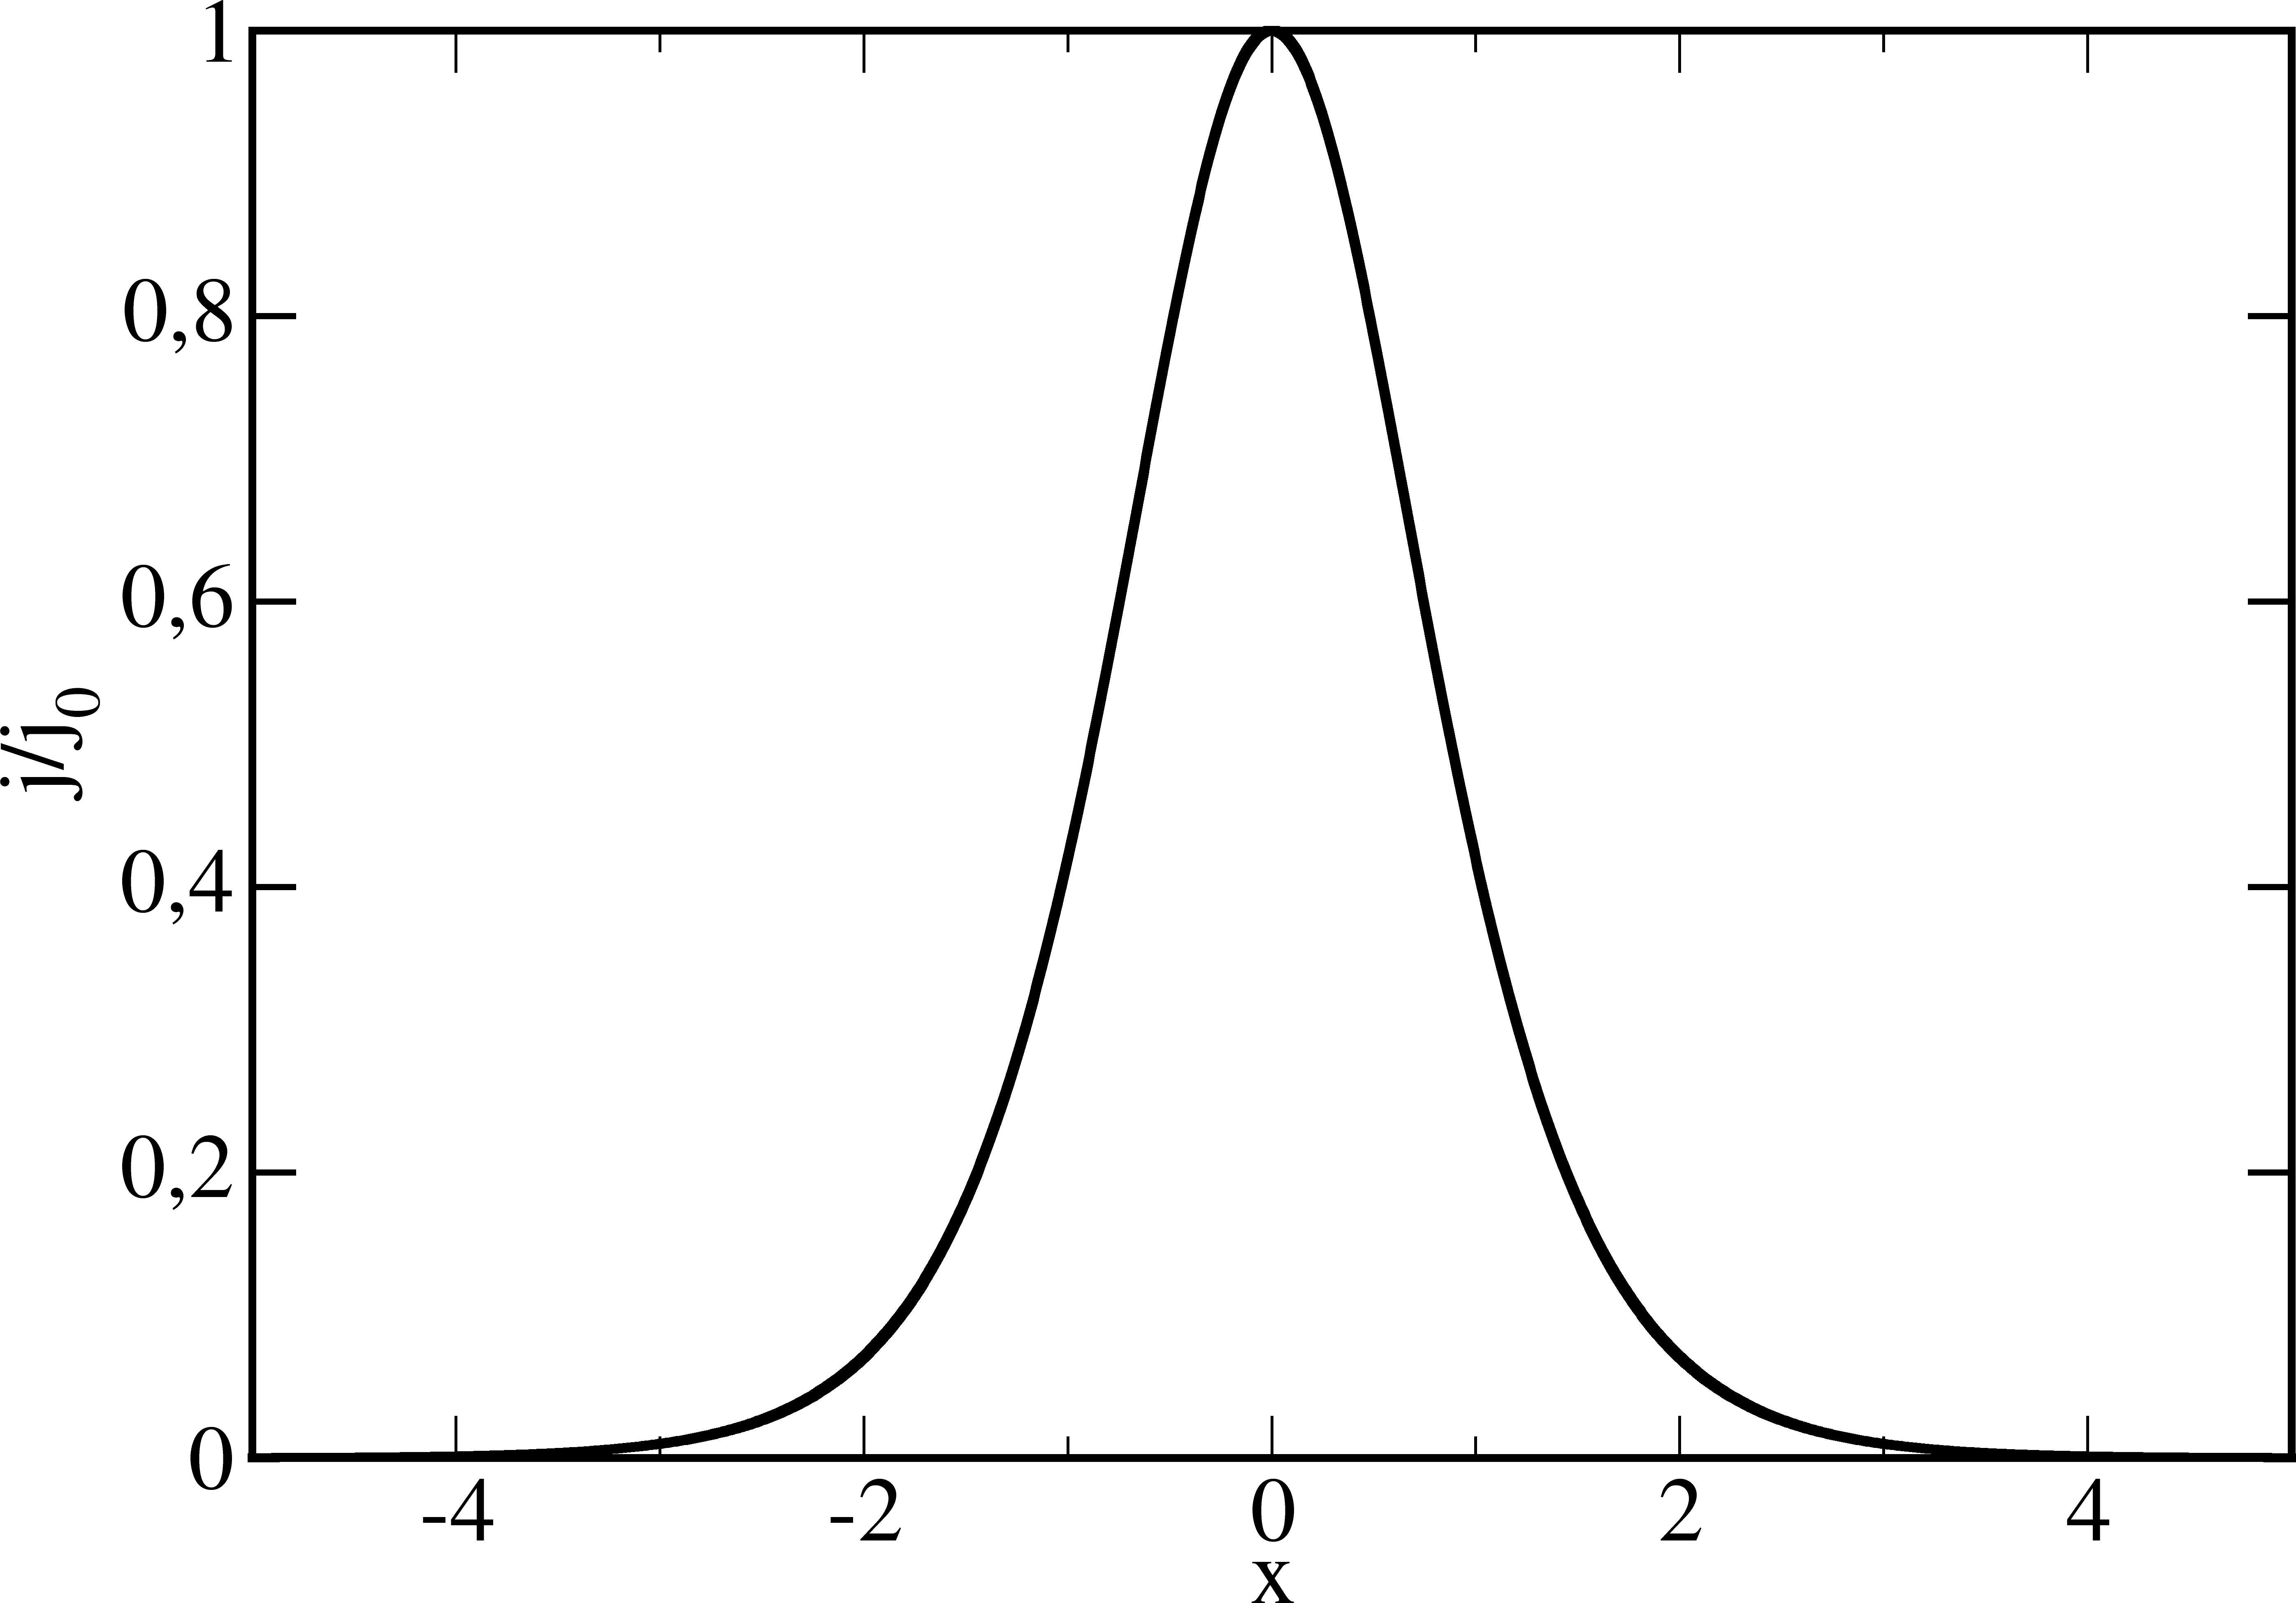
\includegraphics[width=8truecm]{slike/08_soliton.png}
\caption{Prečni profil krajevnega solitona v 2D. Vzdolž koordinate $z$ se profil ohranja.}
\label{fig:soliton}
\end{figure}

Če se vrnemo k izrazu za električno poljsko jakost (enačba~\ref{8.89}), vidimo, da
je parameter $\eta$ nastopa tudi v faznem faktorju. To pomeni, da je od njega odvisna 
tudi konstanta širjenja in s tem fazna hitrost
\index{Soliton!fazna hitrost}
\begin{equation}
v_{f}=\frac{\omega}{k} = \frac{c}{\tilde{n}\left(1+\frac{\eta^{2}}{2k_{0}^{2}}\right)}.
\end{equation}
Fazna hitrost omejenih snopov oziroma solitonov je torej vedno manjša od fazne hitrosti ravnih valov. 
Bolj ko je snop omejen, manjša je fazna hitrost, za velike polmere snopa pa doseže 
limitno vrednost $c_0/\tilde{n}$.

Moč dvodimenzionalnega snopa je enaka integralu
gostote svetlobnega toka (enačba~\ref{8.89a}) po $x$. Integriramo in dobimo 
\begin{equation}
P_S = \int j_s dx \propto \int |E_S|^2 dx  = 
\frac{2}{\kappa}\,\eta^{2}\int_{-\infty}^{\infty}\frac{dx}
{\cosh^{2}\eta x}=\frac{4\eta}{\kappa}.
\label{eq:solj}
\end{equation}
Moč stacionarnega snopa~\textendash~solitona~\textendash~v dveh dimenzijah je 
torej obratno sorazmerna s širino snopa $1/\eta$. Zato tudi pri poljubno veliki moči 
obstaja stacionarna širina. To je bistvena razlika med obravnavanim dvo- in 
tridimenzionalnim primerom, kjer se snop z nadkritično močjo skrči v singularnost.

\section{Optični solitoni}
\index{Soliton!optični}
V prejšnjem razdelku smo ugotovili, da pojav samozbiranja svetlobnega
snopa lahko izniči širjenje zaradi uklona, tako da ima pri
ustrezni moči snop povsod konstantno širino in obliko. Takim snopom 
smo rekli krajevni solitoni. Povsem podoben pojav poznamo tudi v časovni 
domeni, kjer se pojavijo časovni ali optični solitoni. 

Sunek svetlobe  naj se širi po valovnem vodniku. Ker je lomni količnik
odvisen od frekvence valovanja, se sunek svetlobe podaljšuje. Več o tem bomo spoznali pri 
obravnavi disperzije v optičnih vlaknih (poglavje~\ref{chap:Disperzija}). 
Ob primernih pogojih lahko odvisnost lomnega količnika od intenzitete ravno izniči
odvisnost lomnega količnika od valovne dolžine in sunek
ohranja obliko. Sunkom svetlobe, ki potujejo po sredstvu brez spremembe
oblike, pravimo optični solitoni. Posebej so pomembni v optičnih vlaknih, 
kjer je disperzija izrazita in želimo njen vpliv zaradi učinkovitosti prenosa
informacije čim bolj zmanjšati. 

Pojava optičnih solitonov ni težko pojasniti. Naj na optično nelinearno sredstvo
vpade sunek svetlobe, ki je Gaussove oblike (slika~\ref{fig:optsoliton})
\beq
j(t) = j_0 e^{-t^2/\tau^2}.
\label{08_pulz}
\eeq
Faza takega sunka je 
\beq
\phi (t) = k_o n z - \omega_0 t = k_0 (\tilde{n} + n_2 j)z - \omega_0 t = 
\phi_0 + k_0 n_2 z j - \omega_0 t,
\eeq
frekvenca pa 
\beq
\omega = -\frac{d\phi}{dt} = \omega_0 - k_0 n_2 z \frac{dj}{dt}.
\eeq
Če vstavimo časovno obliko sunka svetlobe (enačba~\ref{08_pulz}), vidimo, da se 
frekvenca takega sunka spreminja s časom
\beq
\omega = \omega_0 + \frac{2k_0 n_2 z j_0}{\tau^2} \, t \, e^{-t^2/\tau^2}.
\eeq
Začetnemu delu sunka (pri $t<0$) se torej frekvenca zmanjša, zadnjemu delu sunka
(pri $t>0$) pa se mu poveča (slika~\ref{fig:optsoliton}). 
Ta pojav spreminjanja frekvence znotraj kratkega sunka imenujemo čričkanje sunkov 
({\it chirping}), \index{Čričkanje} po podobnosti z oglašanjem čričkov.

\begin{figure}[h]
\centering
\def\svgwidth{80truemm} 
\input{slike/08_OpticniSoliton.pdf_tex}
\caption{Zaradi nelinearnega lomnega količnika pride do frekvenčnega premika v sunku svetlobe.}
\label{fig:optsoliton}
\end{figure}
Pri prehodu optičnega sunka z osnovno frekvenco $\omega_0$ se torej različnim delom sunka
frekvenca različno spremeni (slika~\ref{fig:chirp}\,a), začetnemu delu se zmanjša, 
zadnjemu pa poveča. Po drugi strani pa v snoveh poznamo barvno disperzijo, 
kar pomeni, da veljajo za valovanja z različnimi frekvencami različni lomni količniki.
\index{Disperzija} Pojav disperzije je še bolj zapleten pri potovanju sunkov svetlobe,
kar bomo podrobneje obravnavali pri optičnih vlaknih (poglavje~\ref{chap:Disperzija}).
Zaenkrat povejmo le, da je pomemben parameter disperzija grupne hitrosti, ki je sorazmerna
z drugim odvodom lomnega količnika po valovni dolžini 
\beq
D = -\frac{\lambda}{c_0}\frac{d^2n}{d\lambda^2}.
\eeq
Pri določenih pogojih (izbrana snov in določeno frekvenčno območje) 
lahko dosežemo, da potuje del valovanja z večjo valovno dolžino hitreje kot del valovanja
z manjšo valovno dolžino (slika~\ref{fig:chirp}\,b). V tem primeru zadnji del sunka 
dohiteva sprednjega in učinek disperzije ravno izniči učinek nelinearnosti. 
Nastane signal, ki ohranja svojo obliko~\textendash~soliton. 
\begin{figure}[h]
\centering
\def\svgwidth{120truemm} 
\input{slike/08_Chirp.pdf_tex}
\caption{Čričkanje sunkov svetlobe zaradi nelinearnega pojava. Z ustrezno disperzijo lahko
čričkanje izničimo in nastane sunek svetlobe, ki oblike ne spreminja~\textendash~soliton.}
\label{fig:chirp}
\end{figure}

\section{*Izpeljava optičnih solitonov}
\index{Soliton!optični}
Za matematični opis optičnih solitonov izhajamo iz nelinearne 
valovne enačbe (enačba~\ref{8.3}), ki jo zapišemo v skalarni obliki
\begin{equation}
\nabla^{2}E-\frac{n^2}{c_0^{2}}{\frac{\partial^2 E}{\partial t^2}}=
\mu_{0}{\frac{\partial^2P_{\textrm{NL}}}{\partial t^2}},
\end{equation}
pri čemer je 
$P_\textrm{NL}$ nelinearna polarizacija tretjega reda (enačba~\ref{eq:nlin3}).
Namesto v časovni domeni je enačbo prikladnejše reševati v frekvenčni domeni, zato
namesto $E$ in $P_{\mathrm{NL}}$ vpeljemo Fourierevi transformiranki $\tilde{E}$ in $\tilde{P}$.
Sledi
\begin{equation}
\nabla^{2}\tilde{E}+\frac{n^2}{c_0^{2}}\omega^2 \tilde{E}=
- \mu_{0}\omega^2 \tilde{P}.
\end{equation}
Gornjo enačbo rešujemo z nastavkoma
\beq
\tilde{E} = \tilde{A} (z,\omega - \omega_0) e^{ik_0z}\quad \textrm{in} \quad 
\tilde{P} = \tilde{B} (z,\omega - \omega_0) e^{ik_0z},
\eeq
pri čemer je $\omega_0$ osrednja frekvenca svetlobnega sunka in $k_0 = \omega_0 n/c_0$. Vpeljemo še
$\Omega =\omega - \omega_0$ in dobimo 
\beq
\left(\frac{\partial^2}{\partial z^2}+k^2\right)\tilde{A}(z,\Omega) e^{ik_0z} =
- \mu_{0}\omega^2 \tilde{B} (z,\Omega) e^{ik_0z}.
\eeq
Da lahko rešimo to enačbo, naredimo nekaj približkov. Ker je $\omega \approx \omega_0$, na desni strani
enačbe nadomestimo frekvenco z osrednjo frekvenco. Poleg tega upoštevamo, da se amplituda 
glede na valovno dolžino le počasi spreminja, zato drugi odvod zanemarimo in 
\beq
2 i k_0 \frac{\partial \tilde{A}}{\partial z} + (k^2-k_0^2) \tilde{A} = - \mu_{0}\omega_0^2 \tilde{B}.
\eeq
Če je disperzija šibka, lahko zapišemo $k^2 - k_0^2$ kot razliko kvadratov, $k(\omega_0 + \Omega)$ pa 
razvijemo v Taylorjevo vrsto okoli osrednje frekvence $\omega_0$ do tretjega člena. Sledi
\beq
k^2 - k_0^2 \approx 2k_0 (k-k_0) \approx 2k_0 (k'\Omega + \frac{1}{2}k''\Omega^2),
\eeq
pri čemer $'$ označuje odvod po frekvenci, in prepišemo enačbo v 
\beq
2 i k_0 \frac{\partial \tilde{A}}{\partial z} + 2k_0(k'\Omega + \frac{1}{2}k''\Omega^2) \tilde{A} 
= - \mu_{0}\omega_0^2 \tilde{B}.
\eeq
Vrnimo se v časovno domeno, tako da naredimo inverzno Fourierevo transformacijo. Naj bo 
$A(z,t)$ kompleksna amplituda električne poljske jakosti in inverzna transformiranka 
funkcije $\tilde{A}(z,\Omega)$, funkcija $B(z,t)$ pa naj bo 
amplituda polarizacije in inverzna transformiranka 
funkcije $\tilde{B}(z,\Omega)$.
Sledi
\begin{equation}
i (\frac{\partial}{\partial z}+\frac{1}{v_{g}}\frac{\partial}{\partial t})A-
\frac{1}{2}\frac{d^{2}k}{d\omega^{2}}\,\frac{\partial^{2}A}{\partial t^{2}}=
-\frac{\mu_0\omega_0^2}{2 k_0}B,
\label{8.93}
\end{equation}
pri čemer smo z $v_g = d\omega/dk = 1/k'$ označili grupno hitrost.
Vpeljimo novo spremenljivko 
\begin{equation}
\tau=t-\frac{z}{v_{g}},
\end{equation}
s katero opišemo obliko sunka $A_S(z,\tau)$, kot ga vidi opazovalec, ki se giblje
z grupno hitrostjo skupaj s sunkom. Uporabimo pravilo verižnega odvajanja in dobimo
\beq
\frac{\partial A}{\partial z} = \frac{\partial A_S}{\partial z} + \frac{\partial A_S}{\partial \tau}
\frac{\partial \tau}{\partial z}
= \frac{\partial A_S}{\partial z} -\frac{1}{v_g} \frac{\partial A_S}{\partial \tau}.
\eeq
Podobno naredimo še za odvod po času $\tau$, ki pa se ne razlikuje od odvoda po času $t$
\beq
\frac{\partial A}{\partial t} = \frac{\partial A_S}{\partial z}\frac{\partial z}{\partial \tau}+
\frac{\partial A_S}{\partial \tau}\frac{\partial \tau}{\partial t} 
= \frac{\partial A_S}{\partial \tau} \qquad \textrm{in} \qquad 
\frac{\partial^2 A}{\partial t^2} = \frac{\partial^2 A_S}{\partial\tau^2}.
\eeq
Vstavimo še amplitudo nelinearne polarizacije (enačba~\ref{eq:ptnl})
\beq
B = \frac{3}{4}\varepsilon_0\chi |A|^2 A.
\eeq
in enačba~(\ref{8.93}) dobi obliko 
\begin{equation}
i\,\frac{\partial A_S}{\partial z}-\frac{1}{2}\frac{d^{2}k}{d\omega^{2}}\,\frac{\partial^{2}A_S}{\partial\tau^{2}}+\kappa\left|A_S\right|^{2}A_S=0,
\label{8.95}
\end{equation}
pri čemer je 
\beq
\kappa = \frac{3\omega_0\chi}{8c_0 \tilde{n}}
\eeq
sorazmeren nelinearnemu lomnemu količniku $n_2$ 
(enačba~\ref{eq:n2}). Enačba~(\ref{8.95}) ni nič drugega kot nelinearna Schr\"odingerjeva 
enačba\index{Nelinearna Schr\"odingerjeva enačba}, ki smo jo 
zapisali že pri izpeljavi krajevnih solitonov~(enačba~\ref{8.84}). Enačbi se razlikujeta v tem, da
ima vlogo prečne koordinate $x$ tukaj čas $\tau$ in rešitve nimajo več konstantnega premera,
ampak imajo konstantno dolžino sunka. Stacionarne rešitve obstojajo le v primeru, kadar je  $d^{2}k/d\omega^{2}<0$ oziroma kadar ima drugi odvod nasprotni predznak od nelinearnega lomnega količnika $n_2$. Kot pri krajevnih solitonih tudi tukaj vpeljemo parameter $\eta$, ki je sorazmeren 
z energijo solitona (enačba~\ref{eq:solj}) in dobimo 
\beq
A_S\left(z,\tau\right)=\sqrt{\frac{2}{\kappa}}\eta\frac{e^{i\eta^{2}z}}{{\cosh}\left(\eta \tau 
\sqrt{2\left|\frac{d^{2}\beta}{d\omega^{2}}\right|^{-1}}\right)}\,
\eeq
\begin{equation}
A\left(z,t\right)=\sqrt{\frac{2}{\kappa}}\eta\frac{e^{i\eta^{2}z}}{{\cosh}\left(\eta (t-\frac{z}{v_g}) 
\sqrt{2\left|\frac{d^{2}\beta}{d\omega^{2}}\right|^{-1}}\right)}.
\label{8.96}
\end{equation}
Zapisana je oblika solitona, ki potuje z grupno hitrostjo in pri tem ohranja obliko. Zaradi tega
so solitoni izredno zanimivi za prenos velike gostote informacij na velike razdalje, saj se izognemo
omejitvam zaradi disperzije. 

\begin{remark}
Ena izmed snovi, ki izpolnjuje pogoj, da je $k''$ nasprotnega predznaka kot $n_2$, so kvarčna 
optična vlakna. Pri valovnih dolžinah vidne svetlobe to sicer ne velja, velja pa za 
$\lambda \gtrsim 1,3~\mu$m.
Pogoj je torej izpolnjen pri valovnih dolžinah okoli 1,5~$\mu$m, ki se navadno uporabljajo 
pri prenosu signalov po optičnih vlaknih in signal lahko potuje brez podaljševanja. 
\end{remark}

\section{Optična fazna konjugacija}
\index{Optična fazna konjugacija}
Optična fazna konjugacija je zanimiv in danes tudi praktično pomemben
pojav, pri katerem nastane iz danega valovanja novo valovanje, ki ima enake valovne
fronte, vendar potuje v nasprotni smeri od prvotnega valovanja. Novo valovanje je torej tako,
kot bi začetnemu valovanju obrnili predznak časa in ga ''zavrteli nazaj''. 

Vzemimo optično nelinearno snov, na katero posvetimo z dvema močnima ravnima
snopoma v nasprotnih smereh. To sta črpalna snopa in njuna valovna vektorja 
naj bosta ${\bf k}_{1}$ in ${\bf k}_2 = -{\bf k}_{1}$. Poleg njiju naj na snov vpada
še tretji, signalni snop, ki ni nujno raven val (slika~\ref{08_OPC1}). 
Signalni snop interferira s prvim črpalnim valom in s tem zaradi nelinearnosti 
tretjega reda povzroči modulacijo lomnega količnika, ki je skoraj periodična, če
je signalni val podoben ravnemu valu. Na tej periodični modulaciji se
drugo črpalno valovanje uklanja, pri čemer je uklonjeno valovanje enake oblike
kot signalno, le potuje v nasprotni smeri, ker ima drugo črpalno valovanje
nasprotno smer od prvega. Črpalni valovanji sta seveda enakovredni in ni
mogoče ločiti, s katerim je signalno valovanje interferiralo in katero se
uklanja.
\begin{figure}[h]
\centering
\def\svgwidth{60truemm} 
\input{slike/08_opc1.pdf_tex}
\caption{Optična fazna konjugacija. Dva močna črpalna žarka (modra) vpadata 
na optično nelinearno snov v nasprotnih smereh, vpadni signal (rdeč) pa se odbije v 
smer, iz katere vpada.}
\label{08_OPC1}
\end{figure}
\begin{remark}Pozoren bralec je ugotovil, da je optična fazna konjugacija zelo 
podobna holografiji, le da pri holografiji najprej zapišemo predmetni snop, 
ki ga kasneje reproduciramo, pri fazni konjugaciji pa zapis začetnega valovanja in 
njegova reprodukcija potekata sočasno. 
\end{remark}

Naj se signalno valovanje razširja v smeri $z$. Potem ga zapišemo kot  
\begin{equation}
E_{3}=\mathrm{Re}\left(A_3\left(z\right)\, e^{i\left(kz-\omega t\right)}\right).
\label{8.97}
\end{equation}
V nadaljevanju bomo pokazali, da je novonastalo valovanje sorazmerno
\begin{equation}
E_{4} \propto \mathrm{Re}\left(A_3^{*}\left(z\right)\, e^{i\left(-kz-\omega t\right)}\right).
\label{8.98}
\end{equation}
Zaradi nasprotnega predznaka $k$ potuje nastalo valovanje v obratni smeri od signalnega
valovanja. Poleg tega je kompleksno konjugirana tudi njegova amplituda. To seveda
ne vpliva na obliko valovnih front, saj so te popolnoma enake kot pri signalnem
valovanju. Zaradi lastnosti, da lahko novo valovanje iz signalnega nastane tako,
da krajevni del kompleksno konjugiramo, nastalemu valovanju pravimo fazno
konjugirano valovanje.
\begin{figure}[h!]
\centering
\def\svgwidth{75truemm} 
\input{slike/08_opc2.pdf_tex}
\caption{Primerjava odbojev na navadnem zrcalu (levo) in faznem konjugatorju (desno): odboj ravnega
vala (a), odboj krogelnega valovanja (b) in odboj popačenega vala (c).}
\label{08_OPC2}
\end{figure}

Uporabna posledica fazne konjugacije je prikazana na sliki~(\ref{08_OPC2}).
Najpreprostejši primer je vpad ravnega vala (a), ki se ne odbije po lomnem zakonu (slika levo),
ampak se odbije v smer, iz katere je vpadel na snov (desno). Drugi primer je krogelni val 
ali v približku tudi Gaussov snop (b). Ko vpade na navadno zrcalo (levo), se njegova divergenca
ohranja in se žarek še naprej razširja. Na fazno konjugiranem zrcalu se kroglast val spet
zbere v izvoru (desno). Tretji primer je poljubno sredstvo, ki valovanju doda naključno
fazo, zato po prehodu valovne fronte niso več gladke (c). Ta popačen snop v faznem
konjugatorju generira fazno konjugiran snop, ki potuje v nasprotni smeri
in ima enako nepravilne valovne fronte kot vpadni val. Po prehodu
skozi nepravilno sredstvo se neravnosti valovne fronte izničijo
in nastanejo enake gladke valovne fronte ravnega vala, kot smo jih imeli na začetku. 
To lastnost popravljanja valovne fronte je mogoče 
koristni uporabiti, na primer namesto enega zrcala v laserskem resonatorju.

\section{*Izpeljava optične fazne konjugacije}
Poglejmo podrobneje, kako v nelinearnem sredstvu nastane fazno konjugiran
val. Kot kaže slika~(\ref{08_OPC1}), je celotno polje v nelinearnem
sredstvu vsota štirih valovanj, dveh močnih črpalnih, signalnega in odbitega
\begin{equation}
E=\frac{1}{2}A_{1}e^{i{\bf k}_{1}\cdot{\bf r}-i\omega t}+\frac{1}{2}A_{2}e^{-i{\bf k}_{1}\cdot{\bf r}-
i\omega t}+\frac{1}{2}A_{3}\left(z\right)e^{ikz-i\omega t}+\frac{1}{2}A_{4}
\left(z\right)e^{-ikz-i\omega t}+{\rm k.k.}
\label{8.99}
\end{equation}
S k.k. smo spet označili kompleksno konjugirane člene.  Vsa valovanja naj imajo
enako frekvenco, zaradi enostavnosti še privzemimo, da so enake tudi vse polarizacije.
Račun poenostavimo še s privzetkom, da sta črpalna vala $E_{1}$
in $E_{2}$ dosti močnejša od $E_{3}$ in $E_{4}$, tako da sta njuni
amplitudi konstantni, $E_{3}\left(z\right)$ in $E_{4}\left(z\right)$
pa se le počasi spreminjata.

Vstavimo $E$ v valovno enačbo z nelinearno polarizacijo (enačba~\ref{8.3}), pri čemer
smo časovni odvod že izvrednotili
\begin{equation}
\nabla^{2}E+\epsilon\frac{\omega^{2}}{c_0^{2}}\, 
E=\mu_{0}\frac{\partial^2 P_{\mathrm{NL}}}{\partial t^2}.
\label{8.100}
\end{equation}
Pri tem je $\epsilon\,\omega^{2}/c_0^{2}=k^{2}$, $P_{\textrm{NL}}$ pa je po enačbi~(\ref{eq:nl3P})
enak $P_\mathrm{NL}= \epsilon_{0}\chi^{(3)}E^3$, kjer je $\chi^{(3)} = \chi$
efektivna nelinearna susceptibilnost
za izbrano polarizacijo vseh polj. 

Ker je $E$ zapisan kot vsota osmih različnih členov
(enačba~\ref{8.99}), vsebuje produkt $E^3$ kar 512 členov. Vendar se njihovo število znatno zmanjša, 
če upoštevamo le tiste z enako časovno odvisnostjo oziroma enako frekvenco.
Poleg tega nas ne zanimajo različne kombinacije valovnih vektorjev, ampak k enačbi za $E_{3}$ 
prispevajo le tisti členi s krajevnim faznim faktorjem $\exp(ikz)$, 
k enačbi za $E_4$ pa tisti z $\exp(-ikz)$. Sledi
\begin{eqnarray}
P_{\mathrm{NL}\,3,4} &=& \frac{1}{8}\varepsilon_0\chi 
\left(6 A_1 A_2 A_4^*+ 6A_1 A_1^*A_3 + 6A_2A_2^*A_3 + 3 A_3A_3^*A_3 + 6 A_4 A_4^* A_3^*\right)
e^{i k z - i\omega t} \nonumber\\
&+& 
\left(6 A_1 A_2 A_3^*+6 A_1 A_1^*A_4 + 6A_2A_2^*A_4 + 6 A_3A_3^*A_4 + 3 A_4 A_4 A_4^*\right)
e^{-i k z - i\omega t}.
\end{eqnarray}
Če zanemarimo še člene, v katerih nastopata $A_3$ in $A_4$ v višjih potencah, dobimo
\begin{eqnarray}
P_{\mathrm{NL}\,3,4} &=& \frac{3}{4}\varepsilon_0\chi 
\left( A_1 A_2 A_4^*+ |A_1|^2 A_3 + |A_2|^2 A_3 \right)
e^{i k z - i\omega t} \nonumber\\
&+& 
\left( A_1 A_2 A_3^*+|A_1|^2 A_4 + |A_2|^2A_4 \right)
e^{-i k z - i\omega t}.
\end{eqnarray}
Vstavimo gornji izraz v valovno enačbo~(enačba~\ref{8.100}) in upoštevamo, 
da se $A_i(z)$ le počasi 
spreminja (kar pomeni, da zanemarimo drugi odvod po $z$). Dobimo enačbi 
\beq
i k \frac{dA_3}{dz} = - \frac{3}{4} \mu_0\varepsilon_0 \chi \omega^2 
\left( A_1 A_2 A_4^*+ (|A_1|^2 + |A_2|^2) A_3 \right)
\label{eq:opc1}
\eeq
in 
\beq
-i k \frac{dA_4}{dz} = - \frac{3}{4} \mu_0\varepsilon_0 \chi \omega^2 
\left( A_1 A_2 A_3^*+ (|A_1|^2 + |A_2|^2) A_4 \right).
\label{eq:opc2}
\eeq
Drugi člen na desni že poznamo: opisuje odvisnost lomnega količnika
od intenzitete črpalnih valov, torej optični Kerrov\index{Kerrov pojav!optični}
pojav, in je zato le dodaten prispevek
k fazi. Vpeljimo novi amplitudi, ki se od prejšnjih razlikujeta zgolj v faznem faktorju.
\beq
\tilde{A}_3 = A_3 \exp\left(-i\frac{ 3 \chi \omega}{4 c_0 n}(|A_1|^2 + |A_2|^2) z\right)
\eeq
in 
\beq
\tilde{A}_4 = A_4 \exp\left(i\frac{ 3 \chi \omega}{4 c_0 n}(|A_1|^2 + |A_2|^2)z\right).
\eeq
Ko novi amplitudi vstavimo v diferencialni enačbi~(enačbi~\ref{eq:opc1} in 
\ref{eq:opc2}), se Kerrov prispevek k fazi ravno odšteje
in dobimo 
\begin{equation}
\frac{d\tilde{A}_{3}}{dz}=i\frac{ 3 \chi \omega}{4 c_0 n}\,
A_{1}A_{2}\tilde{A}_{4}^{*}
\label{8.104}
\end{equation}
in 
\begin{equation}
\frac{d\tilde{A}_{4}}{dz}=-i\frac{ 3 \chi \omega}{4 c_0 n}\,
A_{1}A_{2}\tilde{A}_{3}^*.
\label{8.105}
\end{equation}
Z vpeljavo sklopitvene konstante 
\begin{equation}
\kappa=\frac{ 3 \chi \omega}{4 c_0 n}A_1 A_2
\label{8.106}
\end{equation}
se enačbi poenostavita v
\beq
\frac{d\tilde{A}_{3}}{dz}=i\kappa \tilde{A}_{4}^{*} \qquad
\textrm{oziroma} \qquad \frac{d\tilde{A}^*_{3}}{dz}=-i\kappa^* \tilde{A}_{4} 
\label{8.107a}
\eeq 
in
\begin{equation}
\frac{d\tilde{A}_{4}}{dz}=-i\kappa \tilde{A}_{3}^*.
\label{8.107}
\end{equation}
Tako smo zelo težaven problem nelinearne valovne enačbe prevedli na linearen
sistem dveh preprostih sklopljenih enačb za amplitudi signalnega in
odbitega vala. Splošni rešitvi sistema enačb~(\ref{8.107a}) in (\ref{8.107}) 
sta 
\begin{eqnarray}
\tilde{A}_3^* \left(z\right) & = & C_{1}\cos(\left|\kappa\right|z)+
C_{2}\sin(\left|\kappa\right|z)
\label{8.108}\\
\tilde{A}_4 \left(z\right) & = & D_{1}\cos(\left|\kappa\right|z)+
D_{2}\sin(\left|\kappa\right|z).
\label{8.108a}
\end{eqnarray}
Z upoštevanjem zveze, ki izhaja neposredno iz diferencialne enačbe 
(enačba~\ref{8.107a}), dobimo
\beq
C_1 = \frac{i \kappa^*}{|\kappa|}D_2 \qquad
\textrm{in} \qquad 
C_2 = -\frac{i \kappa^*}{|\kappa|}D_1. 
\eeq
Potrebujemo še robne pogoje za obe valovanji. Z leve, pri $z=0$,
poznamo $\tilde{A}_{3}^{*}\left(0\right)$, pri $z=L$ pa ne more biti odbitega
vala in je zato $\tilde{A}_{4}\left(L\right)=0$. S tem lahko določimo konstanti $D_{1}$
in $D_{2}$
\beq
D_2 = -\frac{i|\kappa|}{\kappa^*} \tilde{A}_3^*(0) \qquad
\textrm{in} \qquad 
D_1 = -D_2 \tan(|\kappa|L). 
\eeq
Gornje enačbe združimo in lahko zapišemo amplitudi znotraj nelinearne snovi
\begin{eqnarray}
\tilde{A}_{3}\left(z\right) & = & \tilde{A}_3(0)
\frac{\cos\left(|\kappa|(L-z)\right)}{\cos\left(|\kappa|L\right)}\\
\tilde{A}_{4}\left(z\right) & = & \tilde{A}_3^*(0)\frac{i \kappa}{|\kappa|}
\frac{\sin\left(|\kappa|(L-z)\right)}{\cos\left(|\kappa|L\right)}
\label{8.109}
\nonumber 
\end{eqnarray}
Izračunajmo še amplitudi odbitega in prepuščenega vala. Amplituda odbitega vala 
pri $z=0$ je 
\boxeq{8.110}{
\tilde{A}_{4}(0)  =  \tilde{A}_3^*(0)\frac{i \kappa}{|\kappa|}
\tan \left(|\kappa|L\right),
}
amplituda prepuščenega pri $z = L$ pa
\boxeq{8.110a}{
\tilde{A}_{3}(L)  =  \frac{\tilde{A}_3^*(0)}{
\cos \left(|\kappa|L\right)}.
}
Oglejmo si gornja rezultata podrobneje. Vidimo, da je odbiti val sorazmeren 
kompleksno konjugirani amplitudi vpadnega vala, kar smo omenili že v prejšnjem
razdelku. Poleg konjugirane amplitude ima tudi natanko nasproten valovni vektor, 
zato tudi ime fazno konjugiran val. Zanimiva je tudi njegova velikost. Ker 
je lahko $\tan\left(|\kappa|L\right)>1$, je odbit val lahko močnejši od vpadnega.
To ojačanje odbitega vala gre seveda na račun moči črpalnih
valov. V našem računu bi lahko amplituda odbite svetlobe narasla proti neskončnosti, 
vendar ne smemo pozabiti, ta zapisane enačbe takrat niso več veljavne, ker smo privzeli, 
da sta signalni in odbiti žarek precej šibkejša od črpalnih.

Poglejmo še prepuščeni žarek. Ker je $\cos(x)\leq1$, je amplituda prepuščenega
žarka vedno večja od amplitude vpadnega. To pomeni, da smo na račun črpalnih žarkov
dobili prepustnost, ki je vedno večja od $100~\%$, in odbojnost, ki je lahko 
večja od $100~\%$.

Doslej smo predpostavili, da je vpadni signal ravni val. Če je njegova
amplituda odvisna še od prečne koordinate, ga lahko razvijemo po ravnih
valovih in zgoraj izpeljana enačba~(\ref{8.110}) velja za vsako komponento posebej. 
Odbite komponente so sorazmerne s konjugiranimi komponentami signalnega valovanja
z nasprotnim valovnim vektorjem in dajo skupaj valovno fronto enake
oblike kot pri signalnem valovanju, le giblje se v nasprotni smeri, kot
smo opisali že na začetku razdelka.

\begin{remark}
Omenili smo že, da se fazno konjugirana zrcala lahko uporabljajo v laserjih, da
izničimo popačenje Gaussovega snopa. Drug primer uporabe je pri optični astronomiji
ali optičnih komunikacijah skozi atmosfero. Naključne spremembe gostote v atmosferi
signalu dodajo naključni fazni premik, ki signal popači. Če se signal odbije od zrcala nazaj
proti izvoru, bo torej dvakratno popačen. Če pa se odbije od fazno konjugiranega zrcala, 
se bo vpliv nehomogenosti atmosfere ravno izničil in na prenos signala ne bo vplival, poleg
tega pa bo šibek signal še dodatno ojačan. 
\end{remark}